\documentclass[final,12pt]{article}
%DIF LATEXDIFF DIFFERENCE FILE
%DIF DEL old.tex             Sat Jul 11 14:22:12 2026
%DIF ADD hermannpopper.tex   Sun Jul 12 10:38:52 2026

\usepackage{els}
\usepackage{ii}
\usetikzlibrary{patterns}
\usepackage{caption}
\captionsetup{font=tiny}
%\RequirePackage{tikz}
%
%\usetikzlibrary{arrows.meta}
%
%\usetikzlibrary{decorations.pathmorphing}
\newcommand{\LdF}{\bt{Logik der Forschung}\xspace}
\newcommand{\Lo}{\bt{Logik}\xspace}
\newcommand{\KPA}[1]{KPA #1}
\newcommand{\TE}{thought experiment\xspace}
\newcommand{\IR}{indeterminacy relations\xspace}
\newcommand{\UR}{uncertainty relations\xspace}
\newcommand{\HR}{Heisenberg's relations\xspace}
\newcommand{\Weis}{Weisskopf\xspace}
\newcommand{\W}{Weizsäcker\xspace}
\newcommand{\vW}{von Weizsäcker\xspace}
\newcommand{\VW}{Von Weizsäcker\xspace}
\newcommand{\CH}{coupling-hypothesis\xspace}
\newcommand{\NW}{\jt{Die Naturwissenschaften}\xspace}
\newcommand{\ERG}{\jt{Erg\"anzung}\xspace}
\newcommand{\fnstar}[1]{\fn{\mbox{\textsuperscript{*}#1}}}

\newcommand{\WH}{\vW-Hermann\xspace}
\newcommand{\HW}{\vW-Hermann\xspace}
\newcommand{\KH}{\german{Kopplungshypothese}\xspace}
\newcommand{\GE}{\german{Gedankenexperiment}}
\newcommand{\LF}[2]{ \autocite[#1/#2]{Popper1935}}
\newcommand{\NGQ}[2]{\autocite[#1/#2]{Hermann1935}}

\newcommand{\pos}{\ensuremath{x}\xspace}
\newcommand{\mom}{\ensuremath{p_x}\xspace}
\newcommand{\pam}{\ensuremath{x} and \ensuremath{p_x}\xspace}

\renewbibmacro*{cite:ibid}{{}}
\renewcommand*{\multicitedelim}{\addsemicolon\space}
%\renewcommand*{ \autocite}{\pipcite}
%\renewcommand*{\footcite}{\pipcite}
%\renewcommand*{ \autocites}{\pipcites}
%\renewcommand*{\footcites}{\pipcites}

\DeclareDocumentCommand\letterKPA{mmmmmo}{%
{\IfNoValueTF {#6}%
{#1 to #2,  \shortmoam\formatdate{#3}{#4}{#5}}%
{#1 to #2,  \shortmoam\formatdate{#3}{#4}{#5}; KPA #6}%
} %
\unspace}

\DeclareDocumentCommand\letterGHp{mmmmmo}{%
\leavevmode\nobreak\unskip
  {(%
    \IfNoValueTF{#6}
      {#1 to #2, \shortmoam\formatdate{#3}{#4}{#5}}%
      {#1 to #2, \shortmoam\formatdate{#3}{#4}{#5}; \cite[Ab.~III, Br. #6]{Herrmann2019}}%
  })%
\unspace}



\DeclareDocumentCommand\letterGH{mmmmmo}{%
{\IfNoValueTF {#6}%
{#1 to #2,  \shortmoam\formatdate{#3}{#4}{#5}}%
{#1 to #2,  \shortmoam\formatdate{#3}{#4}{#5}; \cite[Ab.~III, Br. #6]{Herrmann2019}}%
} %
\unspace}

\DeclareDocumentCommand\letterKPAp{mmmmmo}{%
\leavevmode\nobreak\unskip
  {(%
    \IfNoValueTF{#6}
      {#1 to #2, \shortmoam\formatdate{#3}{#4}{#5}}%
      {#1 to #2, \shortmoam\formatdate{#3}{#4}{#5}; Karl Popper Archives~#6}%
  })%
\unspace}



\DeclareDocumentCommand\letteraep{mmmmmo}{(%
\leavevmode\nobreak\unskip%
{{\IfNoValueTF {#6}%
{#1 to #2,  \shortmoam\formatdate{#3}{#4}{#5}}%
{#1 to #2,  \shortmoam\formatdate{#3}{#4}{#5}; Albert Einstein Archives, #6}%
}%
})\unspace}

\DeclareDocumentCommand\letterae{mmmmmo}{%
{\IfNoValueTF {#6}%
{#1 to #2,  \shortmoam\formatdate{#3}{#4}{#5}}%
{#1 to #2,  \shortmoam\formatdate{#3}{#4}{#5}; Albert Einstein Archives, #6}%
} %
\unspace}

\renewcommand{\rev}[1]{\autocap{R}eview of \citeauthor{#1}, \citetitle{#1}}


\title{Measurement Reconstruction vs.\DIFaddbegin \DIFadd{\ }\DIFaddend Trajectory Reconstruction: \VW between Hermann and Popper}
%DIF < 
%DIF < %\VW between Hermann and Popper: The Early Philosophical Debate on the Past Trajectories of Particles %Measurement Reconstruction vs. Trajectory Reconstruction: \VW between Hermann and Popper
%DIF PREAMBLE EXTENSION ADDED BY LATEXDIFF
%DIF UNDERLINE PREAMBLE %DIF PREAMBLE
\RequirePackage[normalem]{ulem} %DIF PREAMBLE
\RequirePackage{color}\definecolor{RED}{rgb}{1,0,0}\definecolor{BLUE}{rgb}{0,0,1} %DIF PREAMBLE
\providecommand{\DIFadd}[1]{{\protect\color{blue}\uwave{#1}}} %DIF PREAMBLE
\providecommand{\DIFdel}[1]{{\protect\color{red}\sout{#1}}}                      %DIF PREAMBLE
%DIF SAFE PREAMBLE %DIF PREAMBLE
\providecommand{\DIFaddbegin}{} %DIF PREAMBLE
\providecommand{\DIFaddend}{} %DIF PREAMBLE
\providecommand{\DIFdelbegin}{} %DIF PREAMBLE
\providecommand{\DIFdelend}{} %DIF PREAMBLE
\providecommand{\DIFmodbegin}{} %DIF PREAMBLE
\providecommand{\DIFmodend}{} %DIF PREAMBLE
%DIF FLOATSAFE PREAMBLE %DIF PREAMBLE
\providecommand{\DIFaddFL}[1]{\DIFadd{#1}} %DIF PREAMBLE
\providecommand{\DIFdelFL}[1]{\DIFdel{#1}} %DIF PREAMBLE
\providecommand{\DIFaddbeginFL}{} %DIF PREAMBLE
\providecommand{\DIFaddendFL}{} %DIF PREAMBLE
\providecommand{\DIFdelbeginFL}{} %DIF PREAMBLE
\providecommand{\DIFdelendFL}{} %DIF PREAMBLE
%DIF COLORLISTINGS PREAMBLE %DIF PREAMBLE
\RequirePackage{listings} %DIF PREAMBLE
\RequirePackage{color} %DIF PREAMBLE
\lstdefinelanguage{DIFcode}{ %DIF PREAMBLE
%DIF DIFCODE_UNDERLINE %DIF PREAMBLE
  moredelim=[il][\color{red}\sout]{\%DIF\ <\ }, %DIF PREAMBLE
  moredelim=[il][\color{blue}\uwave]{\%DIF\ >\ } %DIF PREAMBLE
} %DIF PREAMBLE
\lstdefinestyle{DIFverbatimstyle}{ %DIF PREAMBLE
	language=DIFcode, %DIF PREAMBLE
	basicstyle=\ttfamily, %DIF PREAMBLE
	columns=fullflexible, %DIF PREAMBLE
	keepspaces=true %DIF PREAMBLE
} %DIF PREAMBLE
\lstnewenvironment{DIFverbatim}{\lstset{style=DIFverbatimstyle}}{} %DIF PREAMBLE
\lstnewenvironment{DIFverbatim*}{\lstset{style=DIFverbatimstyle,showspaces=true}}{} %DIF PREAMBLE
%DIF END PREAMBLE EXTENSION ADDED BY LATEXDIFF

\begin{document}

\maketitle

\DIFaddbegin \begin{abstract}
\DIFadd{Early discussions of }\qm \DIFadd{noted that the }\UR \DIFadd{prohibit exact trajectory predictions but seemed to leave room for retrospective trajectory reconstructions with arbitrarily sharp position and momentum. In his Chicago lectures, Heisenberg treated the physical reality of such reconstructed trajectories as a }\s{matter of taste}\DIFadd{. In 1934, Popper seized on this concession and proposed a }\TE \DIFadd{that, by using conservation laws, sought to turn a sharp }\emph{\DIFadd{trajectory reconstruction}} \DIFadd{into an exact trajectory prediction. Heisenberg and his assistants sharply criticized the proposal. This paper argues that in early 1935 Hermann, drawing on a structurally similar }\TE\DIFadd{, identified Popper's deeper confusion between context-independent trajectory reconstruction and context-dependent }\emph{\DIFadd{measurement reconstruction}}\DIFadd{. It will be shown that the twenty-two-year-old }\vW\DIFadd{, then Heisenberg's assistant, played a pivotal role both in criticizing Popper's arrangement and in providing the thought experiment on which Hermann relied. The paper concludes that, on the eve of the EPR debate, the Hermann--Popper controversy came close to raising the question of whether one may legitimately combine counterfactual attributions of position and momentum into a description of the underlying reality.
}\end{abstract}



%DIF > to a single simultaneous, synchronic state attribution

%DIF > rgued that quantum mechanics permits only context-dependent measurement reconstructions. The twenty-two-year-old \vW, as Heisenberg's assistant \citep{Cassidy2015}, came to occupy a pivotal position in both interpretations of \qm, as discssion partend of Hermann and critique of 
%DIF > 
%DIF >  As the more philosophically inclined member of the Leipzig group, he became Hermann's main discussion partner, suggesting his version of the microscope \TE, which became her tool for analyzing the contextual conditions of measurement. On Popper's side, \vW was the central figure in the Leipzig critical response to Popper's proposed \TE against the \UR in late 1934.


%DIF > \lipsum[1-2]
%DIF > This paper reconstructs an overlooked episode in the early philosophical reception of quantum mechanics: the exchange, mediated by Carl Friedrich von Weizsäcker, between Grete Hermann’s contextual interpretation of measurement and Karl Popper’s defense of particle trajectories. Popper’s 1934 thought experiment tried to use an electron--photon collision, followed by momentum and position measurements, to turn non-predictive trajectory reconstruction into exact prediction. Hermann, drawing on the von Weizsäcker--Hermann $\gamma$-ray microscope and her Leipzig discussions, argued that quantum mechanics permits only context-dependent measurement reconstructions: a registered mark has physical meaning only relative to a definite experimental arrangement. Trajectory reconstructions fail because they combine inferences licensed by mutually exclusive contexts. The paper shows that this disagreement anticipated the later EPR--Bohr dispute over context-independent state attribution in quantum mechanics itself.


\DIFaddend \section*{Introduction}

The status of particles’ past trajectories \DIFdelbegin \DIFdel{proved to be }\DIFdelend \DIFaddbegin \DIFadd{became }\DIFaddend a significant point of contention in the early reception of quantum mechanics. In a letter to his students, Paul Ehrenfest reported an argument that Bohr had used in his discussions with Einstein at the 1927 Solvay conference \letterp{Ehrenfest}{Goudsmit, Uhlenbeck, and Dieke}{3}{11}{1927}\footnote{Cited in \cite[415–418]{Bohr1985}, tr. in \cite[37–41][415–418]{Bohr1985}}. Bohr conceded that one may determine the position of a freely moving body at successive times and \DIFdelbegin \DIFdel{then }\DIFdelend retrospectively calculate its intermediate velocity, and hence its momentum, with arbitrary accuracy. The uncertainty relations therefore appear to be violated. This, however, Bohr continued, is \DIFdelbegin \DIFdel{merely }\DIFdelend a misunderstanding. The momentum at the intermediate time has only been \s{reconstructed}, not actually \s{measured}: \q{The uncertainty principle does not forbid calculating momentum from past data} \letterp{Ehrenfest}{Goudsmit, Uhlenbeck, and Dieke}{3}{11}{1927}. As \posscite[249]{Bohr1928} put it in the published \DIFdelbegin \DIFdel{version of the }\DIFdelend Como lecture, the calculation of the particle’s velocity \DIFdelbegin \DIFdel{during the interval }\DIFdelend between the two position measurements is a mere \s{idealization} from which no meaningful, testable predictions can be derived. 




%See Bohr (1985, pp. 415–418), for the German original and pp.  for the English translation

%Bohr, N. (1985). Collected works. In J. Kalckar (Ed.), Foundations of quantum physics i (Vol. 6) (pp. 1926–1932). Amsterdam: North-Holland.

On page 15 of the German edition of his Chicago lectures, \citet{Heisenberg1930} noted \DIFdelbegin \DIFdel{, somewhat in passing , }\DIFdelend \DIFaddbegin \DIFadd{in passing }\DIFaddend that the decision whether to believe in the physical reality of such past trajectories was, after all, a \s{matter of taste} \origg{Geschmacksfrage}. Heisenberg probably did not anticipate that this cursory remark would become \DIFdelbegin \DIFdel{a source of significant controversy}\DIFdelend \DIFaddbegin \DIFadd{controversial}\DIFaddend . \citet{Schlick1931} was the first to object on philosophical grounds, around the turn of 1931. If such a reconstruction of the past cannot in principle be subjected to possible verification \DIFdelbegin \DIFdel{by means of }\DIFdelend \DIFaddbegin \DIFadd{through }\DIFaddend a testable prediction, then the reality of past trajectories is not a question to be answered as a \s{matter of taste}: the question itself is meaningless. A few weeks later, during a visit to Caltech, Einstein coauthored a short note in which he pressed the issue on physical grounds \citep{Einstein1931-03}. In their two-particle thought experiment, Einstein and his coauthors  \DIFdelbegin \DIFdel{(ETP) }\DIFdelend argued that an exact reconstruction of the past motion of one particle would make it possible, by appealing to the conservation of energy and the geometry of the setup, to predict in advance both the energy and the arrival time of the second particle. This would violate the \UR. \DIFdelbegin \DIFdel{They }\DIFdelend \DIFaddbegin \DIFadd{ETP }\DIFaddend therefore concluded that any such exact reconstruction of the past trajectory must be forbidden.

As \Ehr pointed out to Bohr (\letter{Ehrenfest}{Bohr}{9}{7}{1931}, AHQP/BSC 18), Einstein's thought experiment \DIFdelbegin \DIFdel{was probably the expression of }\DIFdelend \DIFaddbegin \DIFadd{probably expressed }\DIFaddend a deeper concern\footnote{See \cite[Ch.~1]{BacciagaluppiCrull2024} for more detail}: \DIFdelbegin \DIFdel{in }\DIFdelend \DIFaddbegin \DIFadd{by }\DIFaddend virtue of the \UR, the later experimental choice seemed to determine retroactively whether the distant emitted particle possessed a definite energy or a definite time of emission \autocite[see also][]{Einstein1932d}. Schrödinger's notes from this period, written after a talk by Einstein, record the same interpretation. Following a talk in Leiden in November 1931, Ehrenfest may have prompted Einstein to reformulate the argument in terms of position and momentum \letteraep{Einstein}{Ehrenfest}{5}{4}{1932}[10-231]. According to Rosenfeld's recollection, Einstein presented a version of this argument at a talk in Brussels in 1933 \autocite[127--28]{Rosenfeld1967}. If Rosenfeld's recollection is trustworthy, Einstein had already developed something close to the EPR argument before his permanent departure for the United States \DIFdelbegin \DIFdel{in mid-}\DIFdelend \DIFaddbegin \DIFadd{on }\DIFaddend \datemy{17}{10}{1933}.

By that time, the debate over \qm had begun to spread beyond \DIFdelbegin \DIFdel{the circle of }\DIFdelend quantum physicists and into the philosophical discussions of the German-speaking world. \DIFdelbegin \DIFdel{In this context, this }\DIFdelend \DIFaddbegin \DIFadd{This }\DIFaddend broader reception was shaped by an obvious philosophical reference point: Kant's claim that causality is not an \apo contingent regularity discovered by experience, but \DIFaddbegin \DIFadd{an }\DIFaddend \apr necessary condition of the very possibility of scientific experience. It is therefore not surprising that the philosophical discussion of the new theory took the form of the \s{causality debate} \citep[2.VI.1]{Mehra2001a}. The question was not merely whether \qm required a revision of classical mechanics, but whether it had refuted the principle of causality itself \citep{Frank1932}. The uncertainty relations challenge its validity by blocking epistemic access to a particle's future trajectory. The fact that they do not seem, however, to prohibit the reconstruction of past trajectories raised the further question of the particle's ontological status.

In 1933, \citet{Hermann1933} was among the first to enter the debate over causality from the standpoint of the Kantian-Friesian philosophy outlined by Leonard Nelson \citep{Soler2017}. Hermann initially sought to preserve the possibility of a deterministic completion of \qm. Her encounter with Heisenberg's group\footnote{\letter{Weizsäcker}{Hermann}{17}{12}{1933}, \letterunp{Hermann}{Weizsäcker}{14}{1}{1934}; \letter{Weizsäcker}{Hermann}{30}{1}{1934}; \letterGH{Hermann}{Heisenberg}{9}{2}{1934}[457][3,4,6,7]} and her stay at Leipzig in 1934 proved decisive in shifting her point of view. In particular, Heisenberg's assistant Carl Friedrich \vW introduced her to his version of \citets{Heisenberg1927} $\gamma$-ray microscope. \citets{Weizsacker1931} treatment suggested \letterp{Hermann}{Bünning}{23}{5}{1934}\footnote{Archive of the Friedrich Ebert Foundation} that in \qm retroactive inferences are licensed only within definite experimental arrangements: the electron's position can be inferred from the registration of the scattered photon only when the light is brought to an image plane, whereas a focal plane arrangement yields information about the electron's momentum. In this sense, Hermann concluded, \qm does not violate the principle of causality as such; it invalidates only its classical formulation in terms of prediction. Causality is preserved insofar as it allows for \emph{measurement reconstruction}: from a registered mark on a scintillating screen, through the \DIFdelbegin \DIFdel{measuring }\DIFdelend apparatus, back to the definite value of a quantity. 

Popper entered the causality debate on \qm \DIFdelbegin \DIFdel{at about }\DIFdelend \DIFaddbegin \DIFadd{around }\DIFaddend the same time, probably in spring 1934, while completing \LdF \citep{Giovanelli2026}. He aimed to interpret the \IR as statistical dispersion relations and therefore denied that they set an intrinsic limit to the precision of measurements performed on an individual particle. After discussing the matter with Viennese physicists, especially Pauli's assistant Victor Weisskopf, \citet{Popper1934} devised a \TE also based on an electron--photon collision. In a manner not dissimilar \DIFdelbegin \DIFdel{than }\DIFdelend \DIFaddbegin \DIFadd{to }\DIFaddend ETP (but with the opposite goal), Popper argues that if the electron's past path could be reconstructed from a momentum measurement followed by a position measurement, then conservation laws might be used to predict the future position-cum-momentum path of a single photon with arbitrary precision. Popper's argument thus relies on the possibility of \emph{trajectory reconstructions}, which Heisenberg's \s{matter of taste} remark seemed to leave open, and turns it into the basis for trajectory predictions. Popper aimed to show that the reality of particle trajectories cannot be denied, even if \qm provides only statistical laws for them. The principle of causality remains \DIFdelbegin \DIFdel{in place in the form of }\DIFdelend \DIFaddbegin \DIFadd{as }\DIFaddend a postulate: the requirement never to abandon the search for non-statistical laws describing those paths \citep[\S78]{Popper1935}.

Popper and Hermann were born roughly a year apart and shared a \DIFdelbegin \DIFdel{somewhat }\DIFdelend similar Kant-Fries-Nelson philosophical background \citep{Milkov2012}. They were both marginal figures, with little academic track record, although Hermann could rely on much more solid mathematical training. Both entered the causality debate \DIFdelbegin \DIFdel{at about }\DIFdelend \DIFaddbegin \DIFadd{around }\DIFaddend the same time, and they even met in person at the Eighth International Congress of Philosophy, held in Prague in 1934, while \DIFdelbegin \DIFdel{both were in the midst of }\DIFdelend drafting their reflections on the new \qm. Yet they arrived at opposite conclusions. The opposition is especially sharp because their reflections \DIFdelbegin \DIFdel{were centered around }\DIFdelend \DIFaddbegin \DIFadd{centered on }\DIFaddend two thought experiments sharing certain structural similarities. Both Hermann and Popper focused on arrangements in which an electron and a photon collide, so that a quantity of one system can be inferred from a measurement performed on the other \DIFdelbegin \DIFdel{by means of }\DIFdelend \DIFaddbegin \DIFadd{through }\DIFaddend conservation laws. Yet they put this common structure to divergent uses. 

For Hermann, the point of the \TE is to show that \qm requires the \emph{reconstruction of the measurement process}, but that this reconstruction is context-dependent: after an electron--photon collision, once \DIFdelbegin \DIFdel{one chooses to configure the experimental apparatus }\DIFdelend \DIFaddbegin \DIFadd{the apparatus is configured }\DIFaddend to measure either the position or the momentum of the photon, one can determine either the position or the momentum of the electron. For Popper, by contrast, the point of the \TE is to exploit the possibility of \emph{reconstructing the particle trajectory} in order to make a trajectory prediction: after an electron--photon collision, if one can reconstruct both the past position and the past momentum of the electron with arbitrary precision, then, \DIFdelbegin \DIFdel{by means of }\DIFdelend \DIFaddbegin \DIFadd{through }\DIFaddend the conservation laws, one can predict both the future position and momentum of a photon that the quantum formalism describes only statistically. 

The twenty-two-year-old \vW, as Heisenberg's assistant \citep{Cassidy2015}, came to occupy a pivotal position in \DIFdelbegin \DIFdel{the development of both these }\DIFdelend \DIFaddbegin \DIFadd{both }\DIFaddend interpretations of \qm. As the more philosophically inclined \DIFdelbegin \DIFdel{within }\DIFdelend \DIFaddbegin \DIFadd{member of }\DIFaddend the Leipzig group, he became Hermann's main discussion partner, suggesting his version of the microscope \TE, which became her tool for analyzing the contextual conditions of measurement. On Popper's side, \vW was the central figure in the Leipzig critical response to Popper's proposed \TE against the \UR in late 1934. It was \vW who asked Hermann to review \LdF, which had just appeared at the turn of 1935. For this reason, in the final version of her \DIFdelbegin \DIFdel{\mbox{%DIFAUXCMD
\citetitle{Hermann1935b}}\hskip0pt%DIFAUXCMD
}\DIFdelend \DIFaddbegin \DIFadd{\mbox{%DIFAUXCMD
\citetitle{Hermann1935}}\hskip0pt%DIFAUXCMD
}\DIFaddend , finished in March, Hermann included a criticism of Popper's interpretation of \qm that she also developed in her review \citep{Hermann1935a}. Heisenberg and his assistants had dismantled, one after another, each version of the \TE that Popper submitted to them. Hermann tried to get to the heart of the matter. Popper relied on what Heisenberg had unwisely conceded: that the reality of particles' past trajectories might be treated as a \s{matter of taste}. For Hermann, by contrast, the \DIFdelbegin \DIFdel{reconstructions }\DIFdelend \DIFaddbegin \DIFadd{reconstruction }\DIFaddend of such trajectories was impossible as a \s{matter of context}. \emph{Trajectory reconstructions} are impossible because they combine inferences licensed by different and mutually exclusive \emph{measurement reconstructions}.

\DIFaddbegin \DIFadd{With the exception of a few remarks in an otherwise broader-ranging paper by \mbox{%DIFAUXCMD
\citet{Frappier2016}}\hskip0pt%DIFAUXCMD
, however, the Popper-Hermann debate has not been systematically examined nor }\vW\DIFadd{'s role appreciated. }\DIFaddend Popper and Hermann can be understood as proposing two \DIFdelbegin \DIFdel{different }\DIFdelend ways of preserving \emph{causality} after \qm: Popper through the reconstruction of the particle's path, Hermann through the reconstruction of the measurement context. Their thought experiments were presented shortly before Einstein and collaborators published the EPR \TE in May 1935 \citep{Einstein1935}. Each anticipated its structure in a different way \citep[176--181]{Jammer1974}. Both involved correlations between two systems, the use of conservation laws, and the possibility of inferring a quantity of one system by measuring another. With \DIFdelbegin \DIFdel{the appearance of }\DIFdelend Einstein's 1935 paper, however, the center of gravity of the discussion shifted. The EPR discussion showed that the underlying issue was deeper and more general: the problem of \DIFdelbegin \DIFdel{trajectories }\DIFdelend \DIFaddbegin \DIFadd{trajectory }\DIFaddend reconstruction was a special case of the problem of state attribution. Hermann and Popper had discussed context-free \s{trajectories} under the heading of \s{causality}; in retrospect, however, this debate can be seen as a proxy for the Einstein--Bohr dispute over the \s{reality} of context-free \s{states}. In this new context, however, Popper's and Hermann's contributions had very different \DIFdelbegin \DIFdel{destinies}\DIFdelend \DIFaddbegin \DIFadd{fates}\DIFaddend \todo{improve}. 

In correspondence, Einstein managed to convince Popper that his \TE was flawed \letteraep{Einstein}{Popper}{11}{9}{1935}[19-130]. Popper did not return to \qm in a sustained way until the late 1950s \citep{DelSanto2019}, when he began to suggest that the EPR setup could replace his original arrangement in demonstrating the possibility of reconstructing past trajectories with arbitrary precision. Hermann’s \TE, by contrast, may be regarded as one of the earliest philosophical articulations of the line of response later developed in Bohr’s and Heisenberg’s reactions to EPR \citep[sec.~4.4]{BacciagaluppiCrull2024}. Popper’s pronouncements on \qm, dismissed by the Leipzig group as the work of a physical \textit{ignoramus}, became part of the oeuvre of a philosopher whose reputation \DIFdelbegin \DIFdel{only }\DIFdelend grew after the war. Hermann’s philosophical framework \citep{Reichenberger2026}, by contrast, did not survive as a compelling general philosophy of science. Although taken very seriously in Leipzig, her penetrating and technically informed interpretation of \qm faded along with her philosophical framework, only to be rediscovered recently \DIFdelbegin \DIFdel{\mbox{%DIFAUXCMD
\citepp{Crull2017}{Crull2022}}\hskip0pt%DIFAUXCMD
}\DIFdelend \DIFaddbegin \DIFadd{\mbox{%DIFAUXCMD
\citepp{Crull2017}[][see also]{Crull2022}{Cuffaro2022}{Reichenberger2026}}\hskip0pt%DIFAUXCMD
}\DIFaddend . The tables, however, now seem to have turned. Whereas Popper’s attack on the Copenhagen interpretation has largely become a \DIFdelbegin \DIFdel{matter of }\DIFdelend historical curiosity \citep{Howard2012}, Hermann’s interpretation of \qm has gained new visibility as one of \DIFdelbegin \DIFdel{the }\DIFdelend \DIFaddbegin \DIFadd{its }\DIFaddend most sophisticated and coherent expressions \DIFdelbegin \DIFdel{of that interpretation }\DIFdelend \citep{Bacciagaluppi2025}.





%DIF < The central question in the EPR debate is whether it is legitimate to move from two counterfactual attributions of position and momentum to a single simultaneous, synchronic state attribution: EPR answers yes, whereas Bohr answers no. The corresponding question in the Popper–Hermann debate is whether it is legitimate to move from such counterfactual attributions to the reconstruction of a single diachronic trajectory: Popper answers yes, whereas Hermann answers no.
\DIFdelbegin %DIFDELCMD < 

%DIFDELCMD < %%%
\DIFdelend %Popper’s pronouncements on \qm, dismissed by the Leipzig group as the work of a physical \textit{ignoramus}, entered the oeuvre of a philosopher whose reputation grew after the war. Hermann’s philosophical framework \citep{Reichenberger2026}, by contrast, faded from view, taking with it her technically informed interpretation of \qm. Despite being taken seriously in Leipzig, it largely disappeared until its recent rediscovery \citepp{Crull2017}{Crull2022}. The tables have now turned: Popper’s attack on the Copenhagen interpretation has become largely a historical curiosity \citep{Howard2012}, whereas Hermann’s interpretation of \qm is increasingly recognized as one of its most sophisticated and coherent formulations \citep{Bacciagaluppi2025}.

 \section{Popper's 1934 \TE Against the \UR}
%
In November 1934 Arnold Berliner, the editor of \NW, sent Heisenberg the galley proofs of a short note on the \UR \DIFdelbegin \DIFdel{drafter by at that time }\DIFdelend \DIFaddbegin \DIFadd{drafted by a then }\DIFaddend unknown Viennese philosopher. The note proposed a thought experiment \DIFdelbegin \DIFdel{intended }\DIFdelend \DIFaddbegin \DIFadd{meant }\DIFaddend to show that Heisenberg's inequalities 

\begin{equation*}
\Delta \mom \cdot \Delta \pos \geqq \frac{h}{4 \pi}
\end{equation*}
%
could not simply be interpreted as limits on the accuracy of all possible measurements. Popper's starting point is the distinction between measurements \DIFdelbegin \DIFdel{that can be used }\DIFdelend \DIFaddbegin \DIFadd{usable }\DIFaddend for testable predictions and \s{non-predictive} measurements \origg{nichtprognostische Messungen}. The usual thought experiments supporting the uncertainty relations, he claims, show only that certain more accurate measurements cannot be used for subsequent predictions. They do not show, without further argument, that every measurement of position and momentum is subject to the same restriction \citep{Popper1934}.

\subsection{Popper's Thought Experiment}

Popper's proposed experimental arrangement (\cref{fig:P}) consists of two crossed beams. An electron beam $A$ and a light, X-ray, or $\gamma$-ray beam $B$ intersect at $S$. The beam $A$ is assumed to be a monochromatic parallel beam, and hence a plane wave. The beam $B$ passes through a narrow slit at $B_1$ and forms monochromatic spherical waves. Popper therefore treats both $A$ and $B$ as \s{pure cases} \origg{reine Fälle}. He then considers a \q{mental} or \q{imagined} selection of two narrow partial beams $[A]$ and $[B]$ \DIFdelbegin \DIFdel{that intersect }\DIFdelend \DIFaddbegin \DIFadd{intersecting }\DIFaddend at $S$. These partial beams are not technically isolated from the larger beams by diaphragms or other devices, but are selected only in thought.

The momentum $\mathfrak{a}_1$ of the electrons in $A$ is known, \DIFdelbegin \DIFdel{and }\DIFdelend \DIFaddbegin \DIFadd{as is }\DIFaddend the magnitude $|\mathfrak{b}_1|$ of the momentum of the light quanta in $B$\DIFdelbegin \DIFdel{is also known}\DIFdelend . Hence, for the two \s{mentally} selected partial beams $[A]$ and $[B]$, Popper assumes that the momentum vectors $\mathfrak{a}_1$ and $\mathfrak{b}_1$ before a possible collision at $S$ are known. One then considers those electrons in $[A]$ that, after the collision, travel in the direction $SX$. In the Compton effect, a high-energy light quantum transfers part of its momentum to an electron. If one knows the electron's momentum $\mathfrak{a}_2$ after the collision, the momentum vector $\mathfrak{b}_2$ of the light quantum in $[B]$ that collided with it at $S$ can be determined from momentum conservation: $\mathfrak{b}_2=(\mathfrak{a}_1+\mathfrak{b}_1)-\mathfrak{a}_2.$

\begin{figure}
\centering
 \includegraphics[scale=1, trim = 0mm 0mm 0mm 0.8mm, clip]{Popper1934Experiment}
 \caption{from \citet{Popper1934} \label{fig:P}}
\end{figure}

To determine $\mathfrak{a}_2$, Popper places a registering apparatus at $X$. In the 1934 note, he describes it as \qt{an appropriately constructed point counter}{entsprechend konstruierter Spitzenzähler} \citep[807]{Popper1934}. The term \s{point counter} \origg{Spitzenzähler} usually designates a Geiger-type counter that provides a relatively sharp practical determination of the place and time of a particle's passage. Popper, however, gives no technical details and \DIFdelbegin \DIFdel{merely }\DIFdelend assumes that an appropriately modified device could register both the magnitude of the momentum of the electrons arriving from the direction $SX$ and their time of arrival. For each registered value of $|\mathfrak{a}_2|$, Popper claims that one can reconstruct the electron's trajectory and determine the collision point $S$, which varies along the line $SX$ with $|\mathfrak{a}_2|$. Together with the registered \DIFdelbegin \DIFdel{time of arrival }\DIFdelend \DIFaddbegin \DIFadd{arrival time}\DIFaddend , this reconstruction also determines the time of the collision. The position of the corresponding light quantum in $[B]$ at that time is therefore known, and its momentum $\mathfrak{b}_2$ after the collision can be calculated from momentum conservation. With this information, one can predict \DIFdelbegin \DIFdel{the time at which the }\DIFdelend \DIFaddbegin \DIFadd{when the }\DIFaddend light quantum will arrive at $Y$, thereby predicting both its position and momentum with arbitrary precision.

The decisive premise is that the accuracy of non-predictive measurements, that is\DIFaddbegin \DIFadd{, }\DIFaddend the reconstruction of the past trajectory along $SX$\DIFaddbegin \DIFadd{, }\DIFaddend is not, in principle, subject to a restriction of the kind expressed by the uncertainty relations. Popper formulates this as a conditional assumption: he presupposes that the momentum magnitude and \DIFdelbegin \DIFdel{the time of arrival of }\DIFdelend \DIFaddbegin \DIFadd{arrival time of }\DIFaddend an incoming particle can both be measured with arbitrary accuracy in a \emph{non-predictive measurement}. He does not defend this premise in the note, but refers to a discussion elsewhere. The resulting determination of the position and momentum of the $B$-particle, however, has the character of a \emph{predictive measurement}. One can place a second registering apparatus at $Y$, on the path of the $[B]$ particles scattered with the calculated momentum vector $\mathfrak{b}_2$, and test whether the predicted impacts occur at the calculated time. The experiment is thus \DIFdelbegin \DIFdel{intended }\DIFdelend \DIFaddbegin \DIFadd{meant }\DIFaddend to show that exact predictive measurements are possible, given the possibility of exact non-predictive measurements of position and momentum.

Popper emphasizes, however, that the arrangement does not allow one to assign an arbitrarily definite position and momentum to selected individual particles. The particles whose paths are predicted occur at randomly distributed intervals, and they cannot be technically isolated from the swarm of \DIFdelbegin \DIFdel{other }\DIFdelend particles with randomly varying state quantities. The experiment therefore provides no means of producing a collection of particles more homogeneous than a \s{pure case}. This qualification is central to Popper's intended conclusion. If Heisenberg's inequalities are interpreted statistically, as dispersion relations \origg{Streuungsrelationen}, then the experiment does not undermine them. It does not produce an ensemble of $B$ particles all having both sharp position and sharp momentum. If, however, the inequalities are interpreted as accuracy limits \origg{Ungenauigkeitsrelationen} on measurements of individual particles, Popper claims that the thought experiment reveals their inadequacy. Exact predictions concerning individual particles appear possible, even though the statistical interpretation of quantum mechanics remains untouched.

\DIFdelbegin %DIFDELCMD < \subsection{\VW's Obection}
%DIFDELCMD < %%%
\DIFdelend \DIFaddbegin \subsection{\VW's Objection}
\DIFaddend %
Heisenberg wrote to Popper on \datedm{23}{11}{1934}, explaining that, at Berliner's request, he had discussed the note with his assistant \vW. They \DIFdelbegin \DIFdel{subsequently }\DIFdelend \DIFaddbegin \DIFadd{then }\DIFaddend sent Berliner \vW's brief rejoinder and asked him to forward it to Popper: \DIFdelbegin %DIFDELCMD < \q{You will then see what kind of criticism it is. Essentially, it concerns the concept of the \s{non-predictive measurement,} which in our view appears to be misunderstood in your work.}%%%
\DIFdelend \DIFaddbegin \q{You will then see what kind of criticism it is. Essentially, it concerns the concept of the \s{non-predictive measurement,} which in our view appears to be misunderstood in your work}\DIFaddend \letterKPAp{Heisenberg}{Popper}{23}{11}{1934}[305-32]. Heisenberg asked Popper whether he agreed with \vW's considerations and expressed confidence that an agreement could be reached. Popper, who at the time had only one short publication to his name, was still unknown, and it is therefore quite remarkable that Heisenberg chose to engage with him, enlisting \vW for the purpose---the most philosophically inclined of his collaborators.


%The experiment described by Mr. Popper, when discussed correctly, does not permit one to fall below the limit of accuracy given in the uncertainty relation. It is not possible to determine precisely from the measurements in X the place and time of the collision in S. To see this, however, it is necessary to provide precise information about the nature of the measurements in X. Suppose, for example, that first the momentum of the A-particle is measured and then the time of its arrival at a given place. The position measurement does indeed destroy the knowledge of the momentum after the collision; by contrast, from the momentum before the collision and the position, a “trajectory” of the particle before the collision can be constructed. This fact is presumably what Mr. Popper intends to express by the concept of a “non-prognostic measurement.” This trajectory, however, is in principle uncontrollable. For it holds only for the time interval between the end of the momentum measurement and the beginning of the position measurement, during which the particle has no interaction at all with its environment, and it cannot be extended back into the period before the momentum measurement, since the latter in turn destroys the knowledge of the position in accordance with the uncertainty relation.

%The position measurement does indeed destroy the knowledge of the momentum after the collision; by contrast, from the momentum before the collision and the position, a \q{trajectory} \origg{Bahn} of the particle before the collision can be constructed. \q{This trajectory, however, is in principle uncontrollable} \citep{Weizsäcker1934}.

First, \vW dismisses the modified tip counter as a suitable device for measuring momentum at $X$ and suggests \DIFdelbegin \DIFdel{instead }\DIFdelend a scattering method \DIFaddbegin \DIFadd{instead}\DIFaddend . By measuring the Doppler frequency shift $\delta\nu$ of a light quantum scattered by the electron at $X$, one could infer the electron's momentum \DIFdelbegin \DIFdel{on the basis of }\DIFdelend \DIFaddbegin \DIFadd{from }\DIFaddend energy and momentum conservation. The momentum measurement could then be followed by a tip counter and a clock mechanism recording the electron's position and \DIFdelbegin \DIFdel{time of arrival }\DIFdelend \DIFaddbegin \DIFadd{arrival time}\DIFaddend . With this arrangement, \vW concludes, the electron's \s{trajectory} can be reconstructed only for the interval \emph{between} the completion of the momentum measurement and the subsequent registration of position and time; it cannot be extended to the interval \emph{before} the momentum measurement.

The difficulty is that measuring momentum by \DIFdelbegin \DIFdel{means of }\DIFdelend the Doppler effect requires determining the frequency of the scattered radiation with an uncertainty $\Delta \nu$ over a finite observation time $\Delta t$. A highly precise frequency determination requires observing many oscillation periods, \DIFdelbegin \DIFdel{thereby }\DIFdelend making the time of the scattering interaction correspondingly uncertain. Greater precision in the momentum measurement therefore entails less precision in determining when that measurement occurred. Because the electron's velocity changes during the scattering process, its mean velocity over the duration of the momentum measurement is not exactly known. Consequently, even if its position after the momentum measurement is determined exactly, its position before that measurement cannot be inferred with arbitrary accuracy. The collision time at $S$ therefore remains uncertain, and the subsequent trajectory of the corresponding $B$-particle cannot be predicted with arbitrary precision. \VW concludes:

\qt{This trajectory, however, is \emph{in principle} uncontrollable. It is valid only for the time interval between the end of the momentum measurement and the beginning of the position measurement, during which the particle has no interaction whatsoever with its surroundings, and it cannot be extended into the period before the momentum measurement, since the latter itself destroys the knowledge of the position in accordance with the uncertainty relation. \textelp{} Thus, even if the position [at $X_2$] after the momentum measurement is exactly known, one still cannot infer the position \emph{before} the momentum measurement [at $X_1$] with an accuracy greater than the error $h / 4 \pi \Delta p$. That is, our knowledge of the trajectory of particle $A$ before the momentum measurement at $X$, and thus also of the trajectory of particle $B$ after the collision at $S$, is in accordance with the uncertainty relation}{Diese Bahn ist jedoeh prinzipiell unkontrolIierbar. Sie gilt n~imlich nur ffir das Zeitintervali zwischen dem Ende der Impulsmessung und denl Beginn der Ortsmessung, in dem das Teilchen iiberhaupt keine Weehselwirkung mit seiner Umgebung hat, und EiBt sich nieht in den Zeitraum vet der Impulsmessung fortsetzen, da diese ihrerseits die Kenntnis des Orts gem/ifl der Ungenauigkeitsrelation zerstSrt. }[ \autocite[\VW in][808]{Popper1934}]
%
\VW concedes that this demonstration applies only to the \emph{specific} experimental arrangement he has described. He nevertheless sees no reason to doubt that \emph{any} other combination of measuring devices at $X$ would yield the same result. In his view, Popper fails to distinguish between the \s{non-predictive measurements} he has defined and verifiable inferences about the past. Popper's \s{non-predictive measurements} evade the uncertainty relations only because the statements reporting their results do not describe physically possible measurements. Verifiable inferences about the past, by contrast, remain subject to the same accuracy limits as verifiable predictions about the future, given the time-reversal symmetry of the laws of quantum mechanics.\DIFdelbegin %DIFDELCMD < \todo{improve this.}
%DIFDELCMD < %%%
\DIFdelend \DIFaddbegin \todo{improve this}
\DIFaddend 

 
%DIF < The former escape the \IR because they are not physical measurements at all, insofar as they cannot be used as initial conditions for existing dynamical laws to make testable predictions. The latter, by contrast, do satisfy the \IR, which von Weizsäcker regarded as symmetric for the past and the future.
 \DIFdelbegin %DIFDELCMD < 

%DIFDELCMD <  %%%
%DIF < Popper's counterargument is indeed based on a modification of the momentum measuring that he already proposed in Appendix~VI of the \LdF. Popper was surprised at Heisenberg and \vW's reaction. He considered the possibility of reconstructing post trajectories as obvious given that \citep{Heisenberg1930}, on p.~15 in his textbook, concedes that the belief in the existence of such trajectories was a \s{matter of taste} and was not forbidden by the \UR.
%DIF < 
%DIF < Popper must have realized early on that the tip counter was not the right measuring apparatus and that \vW\ was right that a better way was to measure the momentum \emph{measurement} at $X$ via the Doppler effect, that is, by using a collision with a light quantum. According to Popper, however, the latter method has the drawback that it \q{disturbs the particle's momentum (recoil),} so that \qt{the exact instant of the disturbance is not known}{den Impuls des Teilchens stört (Rückstoß) und daß, da der genaue Zeitpunkt der Störung nicht bekannt ist.} \autocite[406]{Popper1934b}. Indeed, no reconstruction of the trajectory before the scattering event at $X_1$ is possible in this way. However, following the same argument he had developed in Appendix VI, Popper suggests that one can resort to \q{a momentum \emph{selection} (electron spectrometer, light filter),} which \qt{unlike the momentum measurement of individual particles, for example by means of the Doppler effect---has the property of not affecting the momenta or momentum components of the selected particles.}{eine Impuls\emph{aussonderung} (Elektronenspektralapparat, Lichtfilter) hat nämlich- im Gegensatz zu der Impulsmessung individueller Teilchen, etwa mit Hilfe des Dopplereffektes - die Eigenschaft, die Impulse bzw. die Impulskomponenten der ausgesonderten Teilchen nicht zu beeinflussen} \autocite[406]{Popper1934b}. If $[A]$ is an electron beam, one can use a spectra analyzer; in this case \qt{only electrons with a certain \myemph{predetermined} amount of momentum enter the Geiger counter}{nur Elektronen mit einem gewissen vorgegebenen Impulsbetrag in den Spitzenzähler einfallen}. 
%DIFDELCMD < 

%DIFDELCMD < %%%
%DIF < If $[A]$ is a light beam, the filter lets through only those light quanta that \emph{already} possessed the required momentum before entering it  \autocite[406]{Popper1934b}.\todo{selfplagiarism}
%DIFDELCMD < 

%DIFDELCMD < %%%
%DIF < \VW\ began by clarifying that he had not intended to disparage Popper or his book, though he maintained his substantive criticism of Popper's notion of a \s{non-prognostic measurement}. In his view, that notion conflicted with the foundations of quantum mechanics as understood by Heisenberg and himself.\letterKPAp{Von Weizsäcker}{Popper}{6}{12}{1934}[360-21]
%DIFDELCMD < 

%DIFDELCMD <  
%DIFDELCMD <  
%DIFDELCMD < %%%
\DIFdelend \section{The Popper-\vW Correspondence}

Popper replied on \datedm{26}{11}{1934}, feeling that he had not been taken seriously. Drawing \DIFdelbegin \DIFdel{implicitly on the more detailed }\DIFdelend \DIFaddbegin \DIFadd{on the fuller }\DIFaddend analysis he had provided in \DIFaddbegin \DIFadd{Appendix VI of }\DIFaddend \LdF\DIFdelbegin \DIFdel{, particularly in Appendix VI }\DIFdelend , which he attached to the letter \letterKPAp{Popper}{Heisenberg}{26}{11}{1934}[305-52], Popper argued that the past trajectory of a particle could be determined \DIFdelbegin \DIFdel{through three possible }\DIFdelend \DIFaddbegin \DIFadd{by three }\DIFaddend kinds of non-predictive measurement: \begin{inparaenum}[(a)] \item two position measurements; (b) a momentum measurement followed by a position measurement; or (c) a position measurement followed by a momentum measurement \end{inparaenum}. \VW's considerations applied to cases (a) and (c): in these cases, \DIFdelbegin \DIFdel{it was indeed possible to reconstruct the trajectory }\DIFdelend \DIFaddbegin \DIFadd{the trajectory could indeed be reconstructed }\DIFaddend only for the interval between the measurements. Case (b), Popper insisted, was different:

\DIFdelbegin %DIFDELCMD < \qt{This line of reasoning, as far as I can see, is not entirely correct in one case: case (b), namely, a position measurement preceded by a momentum measurement. Admittedly, if the momentum measurement is performed here (cf. Mr. von Weizsäcker’s note) by irradiating an individual particle with light, then it does indeed \s{disturb} the position, and once again we can carry out the calculation only for the interval between the momentum measurement and the subsequent position measurement. The situation is different, however, if the momentum measurement consists in a momentum selection, for example, in the case of a light beam, by means of a filter, or, in the case of an electron beam, by means of an electric field perpendicular to the direction of the beam (an electron-velocity selector). In this case, we can not only calculate the exact \s{trajectory} for the interval between the two measurements, but also trace it back into the \s{past} (a claim discussed in greater detail in the printed enclosure).}{Diese Ueberlegung stimmt nun, soviel ich sehe, in einem Fall nicht ganz: es ist der Fall (b), also die Ortsmessung mit vorangegangener Impulsmessung. Zwar: wenn die Impulsmessung hier (vgl. Herrn Weizsäckers Note) durch Bestrahlung eines individuellen Teilchens durch Licht vorgenommen wird, so „stört“ sie wohl den Ort, und wir können wieder die Berechnung nur für das Intervall zwischen der Impuls- und der nachfolgenden Ortsmessung durchführen. Anders jedoch, wenn die Impulsmessung eine Impulssonderung ist, – also etwa (im Falle eines Lichtstrahls) durch ein Filter oder (im Falle eines Elektronenstrahls) durch ein elektrisches Feld normal zur Strahlrichtung (Elektrengeschwindigkeitsgerät) bewerkstelligt wird. In diesem Fall können wir die genaue „Bahn“ nicht nur für das Intervall zwischen den beiden Messungen berechnen, sondern in die „Vergangenheit“ zurückverfolgen (eine Behauptung, die in der gedruckten Beilage näher diskutiert wird).}[\letterKPAp{Popper}{Heisenberg}{26}{11}{1934}[305-52]]
%DIFDELCMD < %%%
\DIFdelend \DIFaddbegin \qt{This line of reasoning, as far as I can see, is not entirely correct in one case: case (b), namely, a position measurement preceded by a momentum measurement. Admittedly, if the momentum measurement is performed here (cf. Mr. von Weizsäcker’s note) by irradiating an individual particle with light, then it does indeed \s{disturb} the position, and once again we can carry out the calculation only for the interval between the momentum measurement and the subsequent position measurement. The situation is different, however, if the momentum measurement consists in a momentum selection, for example, in the case of a light beam, by means of a filter, or, in the case of an electron beam, by means of an electric field perpendicular to the direction of the beam (an electron-velocity selector). In this case, we can not only calculate the exact \s{trajectory} for the interval between the two measurements, but also trace it back into the \s{past} (a claim discussed in greater detail in the printed enclosure)}{Diese Ueberlegung stimmt nun, soviel ich sehe, in einem Fall nicht ganz: es ist der Fall (b), also die Ortsmessung mit vorangegangener Impulsmessung. Zwar: wenn die Impulsmessung hier (vgl. Herrn Weizsäckers Note) durch Bestrahlung eines individuellen Teilchens durch Licht vorgenommen wird, so „stört“ sie wohl den Ort, und wir können wieder die Berechnung nur für das Intervall zwischen der Impuls- und der nachfolgenden Ortsmessung durchführen. Anders jedoch, wenn die Impulsmessung eine Impulssonderung ist, – also etwa (im Falle eines Lichtstrahls) durch ein Filter oder (im Falle eines Elektronenstrahls) durch ein elektrisches Feld normal zur Strahlrichtung (Elektrengeschwindigkeitsgerät) bewerkstelligt wird. In diesem Fall können wir die genaue „Bahn“ nicht nur für das Intervall zwischen den beiden Messungen berechnen, sondern in die „Vergangenheit“ zurückverfolgen (eine Behauptung, die in der gedruckten Beilage näher diskutiert wird)}[\letterKPAp{Popper}{Heisenberg}{26}{11}{1934}[305-52]]
\DIFaddend %
At $X$, \DIFdelbegin \DIFdel{an electrostatic analyzer with parallel plates }\DIFdelend \DIFaddbegin \DIFadd{a parallel-plate electrostatic analyzer }\DIFaddend producing a uniform electric field $E$ perpendicular to the beam direction (see \cref{fig:weizsaeckerelectrical} below) filters a sub-ensemble of electrons with the same \emph{predetermined} momentum $\mathfrak{a}_2$ \emph{without changing it}.\LF{220--21}{299--300}. If the momentum remains unchanged, then so does the position,\footnote{Popper argues that otherwise this would imply action at a distance\DIFdelbegin \DIFdel{.}\DIFdelend } although the latter remains unknown. The unknown position may later be revealed by a second measurement at $X$, where a Geiger counter (or a clock-driven moving film strip) records the position and \DIFdelbegin \DIFdel{time of arrival }\DIFdelend \DIFaddbegin \DIFadd{arrival time}\DIFaddend . Since the first momentum measurement leaves the electron's state unchanged, one might think that the electron's past trajectory could be reconstructed not only \emph{between} the two measurements---momentum followed by position---but also \emph{before} the first momentum measurement.

\DIFdelbegin \DIFdel{The time }\DIFdelend \DIFaddbegin \DIFadd{There }\DIFaddend was now too \DIFdelbegin \DIFdel{short }\DIFdelend \DIFaddbegin \DIFadd{little time }\DIFaddend for Popper to prepare a rejoinder. On \datef{30}{11}{1934}, the Note appeared in volume 22 of \NW, together with \vW's critical comment. On \datedm{6}{12}{1934}, Popper sent Heisenberg a second communication \autocite{Popper1934b} in response to \vW, which he hoped to publish. Popper also attached a copy of the \LdF that had \DIFdelbegin \DIFdel{been just printed but still not }\DIFdelend \DIFaddbegin \DIFadd{just been printed but not yet }\DIFaddend distributed. Popper's counterargument \DIFdelbegin \DIFdel{is indeed }\DIFdelend \DIFaddbegin \DIFadd{was }\DIFaddend based on a modification of the momentum \DIFdelbegin \DIFdel{measuring that he }\DIFdelend \DIFaddbegin \DIFadd{measurement }\DIFaddend already proposed in Appendix~VI of the \LdF. On \datedm{6}{12}{1934}, the same day as Popper's letter, \vW\, at Heisenberg's request, drafted a detailed response,\letterKPAp{Von Weizsäcker}{Popper}{6}{12}{1934}[360-21] which Heisenberg forwarded to Popper a few days later on \datedm{10}{12}{1934}. 

\DIFdelbegin \DIFdel{The thrust of }%DIFDELCMD < \vW%%%
\DIFdelend \DIFaddbegin \VW\DIFaddend 's reply \DIFdelbegin \DIFdel{concerned }\DIFdelend \DIFaddbegin \DIFadd{centered on }\DIFaddend Popper's proposed electrostatic analyzer (see \cref{fig:weizsaeckerelectrical})\DIFdelbegin \DIFdel{that Popper has introduced in}\DIFdelend . \VW\ reconstructed it as a deflection experiment in which an electron beam passes between condenser plates $A$ and $B$ under the action of an electric field $E$. Without the field, the beam would follow the direction $DE$; with the field, it is deflected, so that each impact point on the screen $EF$ corresponds to a value of the transverse momentum. For small deflections, the displacement is
\todo{check}
%
\begin{equation*}
y = \frac{eE}{2m}t^2 = \frac{eE}{2m}\frac{l^2}{v^2}.
\end{equation*}
%
Popper's idea was that the impact point would provide a momentum measurement followed by a position measurement. \VW's objection was that the \DIFdelbegin \DIFdel{geometry of the experiment}\DIFdelend \DIFaddbegin \DIFadd{experiment's geometry }\DIFaddend already contains the limits expressed by the uncertainty principle.\DIFdelbegin %DIFDELCMD < \footnoteh{See appendix \cref{app:1} for more details.}%%%
\DIFdelend \DIFaddbegin \footnoteh{See appendix \cref{app:1} for more details}\DIFaddend \letterKPAp{Von Weizsäcker}{Popper}{6}{12}{1934}[360-21]

To infer the momentum from the \DIFdelbegin \DIFdel{point of impact , the path of the electron}\DIFdelend \DIFaddbegin \DIFadd{impact point, the electron's path }\DIFaddend through the field must be fixed with sufficient precision. This requires diaphragms at $D$ (\cref{fig:weizsaeckerelectrical}). But narrowing the diaphragm increases diffraction. If the slit has width $d$, then the transverse spread $\Delta y$ at the detector is constrained both by the \DIFdelbegin \DIFdel{width of the slit }\DIFdelend \DIFaddbegin \DIFadd{slit width }\DIFaddend and by the transverse momentum uncertainty generated by diffraction:
%
\begin{equation*}
\Delta y > d,
\end{equation*}
\begin{equation*}
\Delta y = \frac{\Delta p_y}{mv}l,
\end{equation*}
with
\begin{equation*}
d\Delta p_y \geq h.
\end{equation*}
It follows that
\begin{equation*}
(\Delta y)^2 \geq \frac{h}{mv}l.
\end{equation*}
%
Thus the \DIFdelbegin \DIFdel{very }\DIFdelend diaphragms required to define the beam path blur the \DIFdelbegin \DIFdel{point on the screen }\DIFdelend \DIFaddbegin \DIFadd{screen point }\DIFaddend that is supposed to determine the momentum \letterKPAp{Von Weizsäcker}{Popper}{6}{12}{1934}[360-21]

\begin{wrapfigure}{r}{0.35\textwidth}
\centering
 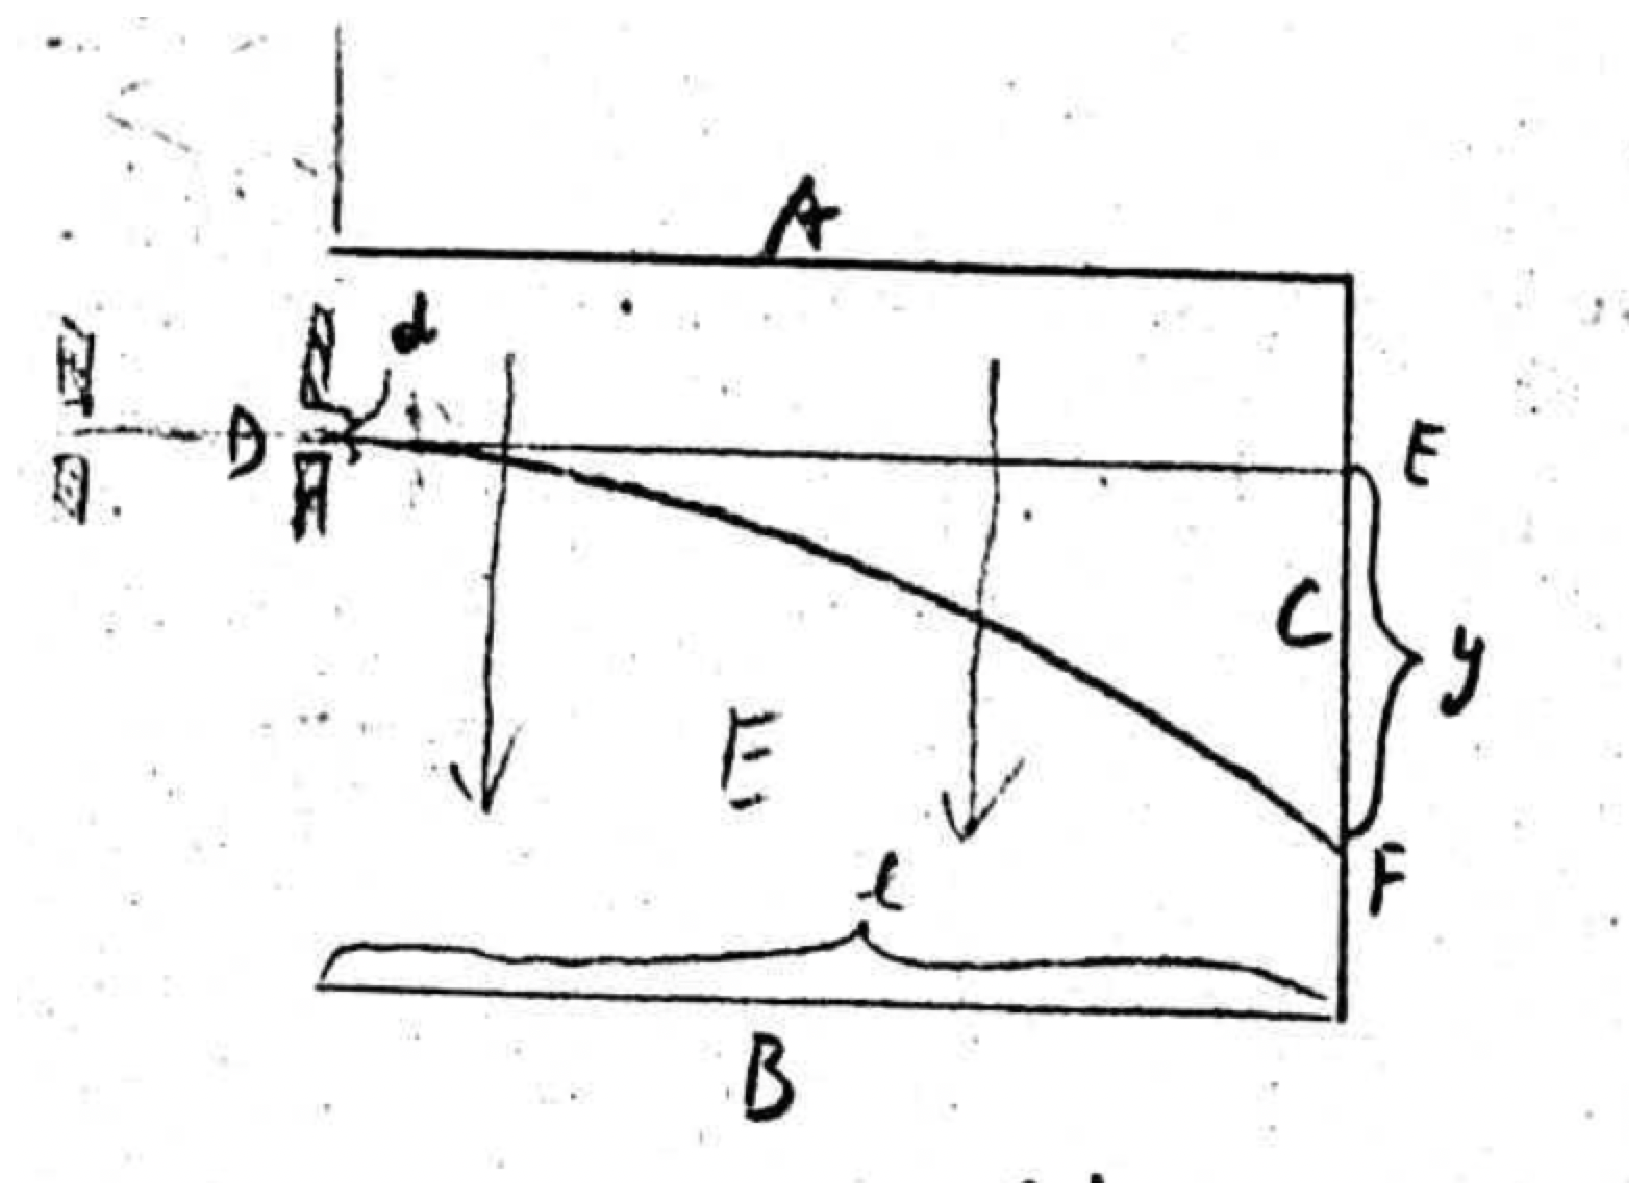
\includegraphics[scale=0.2, trim = 0mm 0mm 0mm 0mm, clip]{1934WeizsaeckerElectrical}
 \caption{From the letter by \letterKPA{von Weizsäcker}{Popper}{6}{12}{1934}[360-21] \label{fig:weizsaeckerelectrical}}

\end{wrapfigure}

This transverse uncertainty also affects the longitudinal motion. Since $y$ depends on the flight time $t=l/v$, an uncertainty in $y$ implies an uncertainty in $v$:
\begin{equation*}
\frac{\Delta y}{y} = 2\frac{\Delta v}{v}.
\end{equation*}
%
This \DIFdelbegin \DIFdel{in turn }\DIFdelend yields an uncertainty in the longitudinal momentum, $\Delta p_x=m\Delta v$, and in the reconstructed coordinate $x=vt$. Combining these uncertainties, \vW\ concluded that the product $\Delta p_x\Delta x$ cannot be \DIFdelbegin \DIFdel{made smaller than }\DIFdelend \DIFaddbegin \DIFadd{reduced below }\DIFaddend the order of Planck's constant. For small deflections, his calculation gives
%
\begin{equation*}
\Delta p_x \Delta x > \frac{l^2}{y^2}h,
\end{equation*}
%
so that no violation of the uncertainty relation is obtained. Larger deflections require an additional angular correction, but do not alter the conclusion.\letterKPAp{Von Weizsäcker}{Popper}{6}{12}{1934}[360-21]
\todo{check}

The decisive point was \DIFdelbegin \DIFdel{therefore }\DIFdelend structural, not merely practical. The same arrangement that makes the impact point interpretable as a momentum measurement also prevents the earlier position from being sharply reconstructed. \VW\ therefore concluded that Popper had not supplied a realizable experiment capable of undercutting the uncertainty principle.\letterKPAp{Von Weizsäcker}{Popper}{6}{12}{1934}[360-21].

% \VW\ stressed that this was the reverse of Heisenberg's example of an initial position determination followed by a momentum measurement in a field. \autocite[21--22]{Heisenberg1930} In both temporal directions, the uncertainty relation blocks the combination of sharp momentum knowledge and retrodictive position knowledge required by Popper's argument. 

%\subsection{Heisenberg's Countereply}
%
%In his reply of \datedm{10}{12}{1934}, Heisenberg enclosed \vW's criticism and opened by assuring Popper that, after discussing the matter with \vW, he had had the note corrected so that it no longer appeared unjustifiably sharp.\letterKPAp{Heisenberg}{Popper}{10}{12}{1934}[305-32] Heisenberg summarized \vW's result as follows: the proposed \s{Aussonderung} of electrons by an electric field is not a genuine momentum measurement in Popper's sense, since the experiment cannot yield an exact trajectory of the particle before the momentum measurement. He then turned to Popper's analogous suggestion of using a light filter instead of an electron spectrometer. As he put it, the optical case could be treated in the same way. The filter would select light of a given frequency, but it would not prepare quanta with an infinitely sharp momentum.
%
%Heisenberg suggested that Popper consider reflective resonance filters, such as sodium or mercury vapor, following Wood's \origg{Reststrahlenverfahren}. Such a device reflects or re-emits radiation near the resonance frequency, while other components of the incident light are not selected in the same way. Thus a broad beam can be reduced, for example, to the sodium D-lines. Yet the selected light is never strictly monochromatic. Since the filtering process depends on the excitation and subsequent de-excitation of the reflecting atom, the resonance line has a finite width. Heisenberg expresses this by writing that the inaccuracy of the momentum of the light quantum is given by
%\begin{equation*}
%\Delta p = \frac{h\Delta\nu}{c^2}.
%\end{equation*}
%The precise form of the factor is less important for his argument than the point that a finite frequency width $\Delta\nu$ entails a finite momentum width $\Delta p$.
%
%Heisenberg then connects this linewidth to a temporal indeterminacy. The probable residence time of the light quantum in the reflecting atom is determined by the lifetime of the corresponding excited state:
%\begin{equation*}
%\Delta t = \frac{1}{\Delta\nu}.
%\end{equation*}
%Thus, even if the later position of the light quantum were known with precision, its position before reflection could not be reconstructed exactly, because the moment at which it was in the reflecting atom remains indeterminate by $\Delta t$. This temporal indeterminacy produces an uncertainty in the reconstructed position before reflection, and Heisenberg concludes that
%\begin{equation*}
%\Delta x \Delta p \sim h.
%\end{equation*}
%In the optical case, therefore, the uncertainty relation is preserved for the same structural reason as in \vW's analysis of the electrostatic analyzer: the physical procedure that selects momentum also prevents an exact retrodiction of the earlier position.
%
%Heisenberg finally made explicit that Popper's \s{nichtprognostischen Messungen} had not, in his view, been shown to be impossible in general merely by \vW's discussion. Rather, what had been shown was that the particular examples Popper had proposed did not work. He nevertheless thought it plausible that the impossibility of such measurements was a very general feature of quantum mechanics. He remarked that a proof of this point would presumably amount to the content of an important paper in mathematical physics, and added that he feared Popper had here followed one of those misleading errors by which he himself, Bohr, and others had been tempted since 1927, before they came to believe that they had really understood quantum theory. He closed by thanking Popper for sending his book, which he had not yet been able to study carefully.\letterKPAp{Heisenberg}{Popper}{10}{12}{1934}[305-32]


% As he put it, the optical case could be treated in the same way. The filter would select light of a given frequency, but it would not prepare quanta with an infinitely sharp momentum, the time of the passage wouild be lost is the time of pasage, since the filter ....  In his reply of \datedm{16}{12}{1934}, 



\DIFdelbegin %DIFDELCMD < \section{The Hermann-Weizäcker Correspondence on Popper's Thought Experiment}
%DIFDELCMD < %%%
\DIFdelend \DIFaddbegin \section{The Hermann-Weizsäcker Correspondence on Popper's Thought Experiment}
\DIFaddend %
In his reply of \datedm{10}{12}{1934}, Heisenberg enclosed \vW's criticism and then dismantled Popper's attempt to invert his \TE \DIFdelbegin \DIFdel{, }\DIFdelend by replacing $[A]$ with a light or Röntgen beam and \DIFdelbegin \DIFdel{to use }\DIFdelend \DIFaddbegin \DIFadd{using }\DIFaddend a light filter, \DIFdelbegin \DIFdel{instead of }\DIFdelend \DIFaddbegin \DIFadd{rather than }\DIFaddend an electron spectrometer, to select light quanta that already possessed the \s{right} momentum \letterKPAp{Heisenberg}{Popper}{10}{12}{1934}[305-32]\todo{check}. Popper sent Heisenberg a revised version of the second communication summarizing the \DIFdelbegin \DIFdel{main points of the }\DIFdelend debate \autocite{Popper1934c}. He conceded that \vW's argument against the electrostatic selector was correct but defended his idea of using a light-quantum filter against Heisenberg's objections \letterKPAp{Popper}{Heisenberg}{16}{12}{1934}[305-32]. Heisenberg did not \DIFdelbegin \DIFdel{further replied}\DIFdelend \DIFaddbegin \DIFadd{reply further}\DIFaddend . By then the Leipzig group had begun to tire of Popper's refusal to let the matter drop. But Popper persisted. He suggested another experimental arrangement, whose examination Heisenberg delegated to his other assistant Hans Euler. Popper envisaged two diffraction gratings inclined in opposite directions, each imposing a separate selection condition, hoping to select both \DIFdelbegin \DIFdel{wave length }\DIFdelend \DIFaddbegin \DIFadd{wavelength }\DIFaddend and direction of the incoming light quanta. Euler replied on \datef{4}{2}{1935} by showing that the two gratings form a single coherent interference system and cannot be treated separately\footnote{Popper--Euler Correspondence, Karl Popper Archives 293-29}. 

\subsection{Hermann's Letter to \VW}
%
During those weeks, \vW received a review copy of \LdF from the \emph{Physikalische Zeitschrift}. Given their dispute in the preceding months, however, he declined to review the book and instead sent it to Hermann. Hermann wrote \vW from Østrupgaard in Denmark to ask for clarification about his response to Popper's \TE \letterGHp{Hermann}{\W}{5}{3}{1935}[14]. In particular, she asked for an offprint of his reply to Popper in \emph{Die Naturwissenschaften}, since she wanted to determine how far Popper had \DIFdelbegin \DIFdel{actually }\DIFdelend responded to his objections. She observes that Popper’s thought experiment in the main text of \LdF appears essentially unchanged from the version he had explained to her in Prague, probably \DIFdelbegin \DIFdel{on the occasion of the }\DIFdelend \DIFaddbegin \DIFadd{at the }\DIFaddend 1934 philosophy congress, and from the version discussed in \emph{Die Naturwissenschaften}. The two appendices, however, seem to her to reflect Popper’s discussion with Weizsäcker \letterGHp{Hermann}{\W}{5}{3}{1935}[14]. This was not in fact the case, since the Appendices $VI$ and $VIII$ had already been written before \vW's response; nevertheless, as we have seen, Popper does seem to have anticipated a possible objection to his momentum-measuring apparatus and had already proposed a momentum filter as a replacement. Hermann, however, pointed out that this would not solve the problem:

\qt{Both \textins{appendices} concern the possibility of detecting a corpuscle in such a way that the position and time of impact, for example on a strip of film or by means of a point counter, are determined precisely, together with the direction and magnitude of the momentum with which the particle arrives. In the first case, the aim is to determine the magnitude of the momentum for a given direction; in the second, to determine the direction as well. What is more, the measurements are supposed to be such that they do not apply merely to the interval \emph{between} the momentum measurement and the position measurement, during which, incidentally, no further disturbance may occur; rather, they are also supposed to determine the exact trajectory of the corpuscle for the time \emph{before} the momentum measurement, so that, on the basis of some earlier collision, the trajectory of another particle can then be predicted with an accuracy exceeding the uncertainty relations. The decisive trick by which this physically inadmissible prediction is to be forced is, in the first appendix \textins{VI}, a momentum selection, that is, a selection of the particles in which this momentum is found, to be carried out on a nonmonochromatic, parallel-directed beam of particles, and specifically in such a way that the momenta of the selected particles, or their momentum component in the direction of the beam, are not changed}{Es geht in beiden um die Möglichkeit, ein Korpuskel derart aufzufangen, dass dabei der Ort und der Zeitpunkt des Auftreffens etwa auf dem Filmstreifen oder mit einem Spitzenzähler1 und zugleich Richtung und Betrag des Impulses, mit dem das Teilchen auftrifft, genau bestimmt wird, im ersten darum, bei gegebener Richtung den Impulsbetrag, im zweiten darum, auch die Richtung festzulegen. Und zwar sollen die Messungen so sein, dass sie nicht etwa nur für den Zeitraum zwischen Impuls- und Ortsmessung gelten, in dem im übrigen keine weitere Störung stattfinden darf, sondern sie sollen auch für die Zeit vor der Impulsmessung die genaue Bahn der Korpuskel bestimmen, sodass dann auf Grund irgend eines früheren Zusammenstosses die Bahn eines anderen Teilchens mit einer die Unbestimmtheitsrelationen übersteigenden Genauigkeit vorhergesagt werden kann. Der entscheidende Trick, mit dem diese physikalisch unzulässige Voraussage erzwungen werden soll, ist im ersten Anhang eine Impul- saussonderung (d. h. Auslese der Teilchen, an denen dieser Impuls angetroffen wird), die an einem nichtmonochromatischen, parallel gerichteten Teilchenstrahl vorgenommen werden soll, und zwar so, dass dabei die Impulse der ausgesonderten Teilchen (bzw. ihre Impulskomponente in der Strahlrichtung) nicht verändert wird}[\letterGHp{Hermann}{\W}{5}{3}{1935}[14]]
%
Hermann clearly identified the central flaw of Popper's arrangements: Popper needs \DIFdelbegin \DIFdel{not only to determine the momentum of the electron}\DIFdelend \DIFaddbegin \DIFadd{to determine not only the electron's momentum }\DIFaddend between the momentum and position measurements, but also \DIFdelbegin \DIFdel{to determine }\DIFdelend its momentum before the first momentum measurement, in order to reconstruct the \DIFdelbegin \DIFdel{time of collision }\DIFdelend \DIFaddbegin \DIFadd{collision time }\DIFaddend at $S$ \DIFdelbegin \DIFdel{, }\DIFdelend and thereby predict the entire trajectory of the correlated particle $B$ \DIFdelbegin \DIFdel{that could be tested }\DIFdelend \DIFaddbegin \DIFadd{testable }\DIFaddend at $Y$.

Hermann jotted down some still \DIFdelbegin \DIFdel{somewhat undeveloped ideas in order }\DIFdelend \DIFaddbegin \DIFadd{undeveloped ideas }\DIFaddend to ask for \vW's opinion\DIFdelbegin \DIFdel{on the matter}\DIFdelend . They are articulated in three points.

\begin{enumerate}
\item Hermann first points out that, according to \qm, Popper cannot use the momentum measurement at $X$ to retrodict the earlier trajectory of the $A$-particle with arbitrary precision. At this point, she tentatively locates Popper's mistake in the assumption that \DIFdelbegin \DIFdel{it is possible to measure }\DIFdelend a momentum component \DIFdelbegin \DIFdel{without taking into account }\DIFdelend \DIFaddbegin \DIFadd{can be measured without }\DIFaddend an uncontrollable disturbance of that very component: \qt{An exact momentum measurement will therefore be able to determine either the momentum before the measurement or the momentum after it, but not both}{Eine genaue Impulsmessung wird also nur entweder den Impuls vor, oder den nach der Messung festlegen können, nicht aber beides} \letterGHp{Hermann}{Weizsäcker}{5}{3}{1935}[14]. Otherwise, she argues, an exact momentum measurement would determine both the momentum before and the momentum after the measurement, thereby immediately violating the uncertainty relations. Yet Hermann does not rest content with this apparatus-specific disturbance argument. She asks whether the impossibility of such a measurement can be derived more generally from the deeper requirement of wave-particle duality. Popper appeals to various devices--a film strip or tip counter for registering the particle, a filter for a light beam, and spectral analysis in an electric field for an electron beam--but Hermann is unsure how, in each case, the failure of the proposed apparatus follows from the necessary interplay of wave and particle descriptions.

\item Hermann then identifies the deeper source of Popper's mistake in his misunderstanding of wave-particle duality. \DIFdelbegin \DIFdel{By reading }\DIFdelend \DIFaddbegin \DIFadd{From }\DIFaddend the \LdF, one can gather that Popper treats the $\psi$-function as a wave-like statistical description not of individual physical systems, but only of ensembles of such systems: \qt{The error in this consideration is this: according to Heisenberg's derivation, the uncertainty relations follow from the dualism experiments and from the compulsion issuing from them to apply features of the wave picture to every atomic process, and features of the corpuscular picture to every wave propagation}{Der Fehler dieser Überlegung: Die Unbestimmtheitsrelationen folgen gemäss Heisenbergs Ableitung aus den Dualismus-Experimenten und der von ihnen ausgehenden Nötigung, auf jeden atomaren Vorgang auch Merkmale des Wellenbildes, auf jede Wellenausbreitung auch Merkmale des Korpuskelbildes anzuwenden} \letterGHp{Hermann}{Weizsäcker}{5}{3}{1935}[14]. The \UR therefore limit not merely the composition of ensembles, but the applicability of classical state descriptions to individual systems. The probability interpretation of the wave function captures only one aspect of \qm: it specifies what can be said when one passes from one measurement context to another. After the momentum measurement, the system is in an eigenstate of the momentum operator; in this case the corresponding value is not merely probable but fixed. But if one asks what would be obtained by measuring position, for instance what position would be found after a momentum context has been fixed, the wave function supplies only a probability distribution over possible outcomes: \qt{Popper fails to recognize this side of Bohr's complementarity}{Diese Seite der Bohrschen Komplementarität verkennt Popper} \letterGHp{Hermann}{Weizsäcker}{5}{3}{1935}[14].

%Relative to a fixed observation context, by contrast, the wave function provides an exact state description, independent of probability statements. 

\item Given these premises, Hermann turns to \DIFdelbegin \DIFdel{the problem of }\DIFdelend past trajectory reconstructions. Popper is not merely unable to reconstruct the trajectory of the $A$-particle before the momentum measurement at $X$; it also makes no sense, in the relevant physical sense, to speak of a particle's trajectory between the momentum and the position measurement. In general, retrospective trajectory calculations are physically meaningless insofar as they combine determinations that belong to different observation contexts. These calculations ignore wave-particle duality by restricting themselves to the intuitive features of only one picture, usually the corpuscular picture, and then \DIFdelbegin \DIFdel{by }\DIFdelend joining together quantities fixed in distinct measurements. The \DIFdelbegin \DIFdel{electron-photon }\DIFdelend \DIFaddbegin \DIFadd{electron--photon }\DIFaddend interaction cannot be described solely as a corpuscular collision. The propagation of the scattered light must be described within the wave picture, while the interaction between the light quantum and the electron is described within the corpuscular picture. The apparatus is therefore needed not merely to register the collision, but to determine how the wave-optical propagation is correlated with the corpuscular scattering event. Optical instruments of this kind fix either the point of origin or the direction of propagation of the scattered light, but not both with arbitrary precision. Hermann here alludes to \vW's $\gamma$-ray microscope. Hermann therefore concludes that Heisenberg’s \qt{much-debated remark}{viel umstrittene Äusserung}, according to which the past trajectory was a matter of taste, was unfortunate.
\end{enumerate}
%
As we shall see, \vW would express some reservations about point (1). Otherwise, however, the letter contained the outline of Hermann's critique of Popper's interpretation of \qm, which she would articulate \DIFdelbegin \DIFdel{both in }\DIFdelend \DIFaddbegin \DIFadd{in both }\DIFaddend her long article on \qm \DIFdelbegin \DIFdel{\mbox{%DIFAUXCMD
\citep{Hermann1935b} }\hskip0pt%DIFAUXCMD
and in }\DIFdelend \DIFaddbegin \DIFadd{\mbox{%DIFAUXCMD
\citep{Hermann1935} }\hskip0pt%DIFAUXCMD
and }\DIFaddend her review of \LdF \citep{Hermann1935a}.

\subsection{\VW's Reply to Hermann}

\begin{wrapfigure}{r}{0.20\textwidth}
\centering
\includegraphics[scale=0.3, trim=0mm 0mm 0mm 0mm, clip]{spitz}
\citetrackerfalse
\caption{From \cite[485]{Herrmann2019}}
\end{wrapfigure}

Hermann’s tone is markedly different from Popper’s self-assured manner. Despite having a much more sophisticated knowledge of \qm, she proceeds cautiously, asking at nearly every step whether \vW would agree with her remarks. \VW thus plays the \DIFdelbegin \DIFdel{role of the }\DIFdelend expert to whom Hermann turns for \DIFdelbegin \DIFdel{clarification on technical matters }\DIFdelend \DIFaddbegin \DIFadd{technical clarification }\DIFaddend \letterGHp{Weizsäcker}{Hermann}{13}{3}{1935}[15]. For instance, at Hermann's request, \vW explains what a tip counter is, an instrument with which Hermann was apparently unfamiliar. In such a counter, the sensitive electrode is a fine metal tip $S$ \origg{Spitze}, maintained at a high potential difference relative to the surrounding conductive wall $W$ of the gas-filled counter chamber. An ionizing particle passing sufficiently close to the tip produces primary ions in the gas; the strong electric field near the tip then amplifies this ionization into a discharge. The discharge registers that a particle has passed through the small sensitive region around the tip and thus gives a relatively sharp practical determination of the place and time of its passage. As \vW adds, \DIFdelbegin %DIFDELCMD < \qt{A photographic plate, pinhole aperture, or the like therefore performs exactly the same function as it does}{Eine photographische Platte, Lochblende o. ä. tut also genau dieselben Dienste wie er} %%%
\DIFdelend \DIFaddbegin \qt{A photographic plate, pinhole aperture, or the like therefore performs exactly the same function as the tip counter}{Eine photographische Platte, Lochblende o. ä. tut also genau dieselben Dienste wie er} \DIFaddend \letterGHp{Weizsäcker}{Hermann}{13}{3}{1935}[15].

\begin{wrapfigure}{l}{0.35\textwidth}
\centering

\includegraphics[scale=0.3, trim=0mm 0mm 0mm 0mm, clip]{vWfilter}
\citetrackerfalse
\caption{from \cite[483]{Herrmann2019}}
\end{wrapfigure}

The system, or any straightforward modification of it, is not suitable for measuring momentum, contrary to Popper's claim. For this reason, in his paper \vW had proposed a measurement by \DIFdelbegin \DIFdel{means of }\DIFdelend the Doppler effect. He agrees with the result of Hermann's critique in point (1) of her letter, but slightly revises her diagnosis of the failure \letterGHp{Weizsäcker}{Hermann}{13}{3}{1935}[15]. On Hermann's diagnosis, an exact momentum measurement cannot determine both the incoming and the outgoing momentum, because the measurement must involve an uncontrollable disturbance of the measured momentum component itself \letterGHp{Weizsäcker}{Hermann}{13}{3}{1935}[15]. According to \vW, however, even if the incoming and outgoing momenta are both known, an exact momentum measurement takes a finite time, so that the instant of the measuring collision is not known. Consequently, a later position cannot be traced back through the measuring process to an earlier position with arbitrary precision. Even granting Popper exact knowledge of the momentum before and after the measuring interaction, he still cannot reconstruct the \DIFdelbegin \DIFdel{time of collision }\DIFdelend \DIFaddbegin \DIFadd{collision time }\DIFaddend at $S$, because he does not know how long the particle moved with the pre-collision momentum and how long \DIFdelbegin \DIFdel{it moved }\DIFdelend with the post-collision momentum \letterGHp{Weizsäcker}{Hermann}{13}{3}{1935}[15].

Popper's selection of electron momenta in an electric field does not improve the situation. \vW reiterates a simplified version of the argument that he and Heisenberg had developed in correspondence with Popper. He adds that Popper's filter has the same structure as the field-deflection measurement discussed by Heisenberg for a magnetic field in his textbook \citep[21--22]{Heisenberg1930}. In Heisenberg's example, a beam of charged particles passes through a slit of width $d$, traverses a homogeneous magnetic field over a distance $a$, and is deflected by an angle $\alpha$, from which the longitudinal velocity, and hence the momentum, can be inferred\DIFdelbegin \DIFdel{according to
}\DIFdelend \DIFaddbegin \DIFadd{:
}\DIFaddend \begin{equation*}
\alpha=\frac{aHe}{mcv}.
\end{equation*}
%
\VW schematizes the same problem by considering a beam entering a field region through an aperture of width $d$ and arriving at a point $P$ after a displacement $y$. The arrival point can function as momentum information only because the field maps different momenta onto different deflections. But this inference presupposes that \DIFaddbegin \DIFadd{an aperture has defined }\DIFaddend the incoming beam\DIFdelbegin \DIFdel{has been defined by an aperture: the finite width of the aperture }\DIFdelend \DIFaddbegin \DIFadd{: its finite width }\DIFaddend limits the geometrical accuracy of the reconstruction, while too narrow an aperture produces diffraction. Heisenberg therefore obtains, for the magnetic-field case, the constraints
\begin{equation*}
\Delta \alpha \gtrsim \frac{d}{l+a} \quad \quad \Delta \alpha \gtrsim \frac{\lambda}{d},
\end{equation*}
%
which jointly prevent an arbitrarily sharp determination of both the beam localization and the direction of propagation. The same limitation applies to \vW's simplified diagram: the later arrival at $P$ and the displacement $y$ do not allow one to reconstruct a precise earlier position independently of the conditions that made \DIFdelbegin \DIFdel{the }\DIFdelend momentum selection possible. In both cases, the field-deflection measurement yields momentum information only at the cost imposed by aperture width and diffraction, so that the uncertainty relation is restored.

Popper had proposed light-filter arrangements as well, but \vW notes that he initially had no clear account of what sort of filter should be used for light. Here again \vW deploys the response that Heisenberg had already given to Popper. One possible realization would be resonance fluorescence: a gas transmits all light except for one spectral line, which, as Wood had shown experimentally, is almost metallically reflected. In this sense, the gas \s{filters out} light quanta with a particular momentum. But this case exhibits the same difficulty as Popper's electron momentum selection. In resonance fluorescence, the atom is temporarily raised to an excited state \DIFdelbegin \DIFdel{, and this excited state has }\DIFdelend \DIFaddbegin \DIFadd{with }\DIFaddend a finite lifetime. The sharpness of the spectral line is connected with the mean lifetime by the uncertainty relation, roughly:
\begin{equation*}
h \Delta \nu \cdot \Delta t \sim h.
\end{equation*}
%
Thus the more sharply the spectral line, or equivalently the photon energy or momentum, is selected, the less sharply the time of the process is determined. The light quantum remains in the atom for a time uncertain by approximately $\Delta t$. This temporal indeterminacy plays the same role as the indeterminate moment of collision in the electron momentum measurement: it prevents one from combining an exact momentum determination with a precise temporal or positional reconstruction. Popper's filter therefore does not evade the uncertainty relations. Even when a filter seems to select a definite momentum component, the process by which it does so involves an uncontrollable temporal indeterminacy. This destroys the possibility of using the filtered photon \DIFdelbegin \DIFdel{as part of }\DIFdelend \DIFaddbegin \DIFadd{in }\DIFaddend a precise trajectory-like reconstruction.

\VW recounts that, after the failure of Popper's first proposals, Popper devised further experimental arrangements. These, however, need not be discussed in detail. For a time, the refutation of Popperian arrangements had become, as \vW put it, \q{a parlor game \origins{Gesellschaftsspiel} for us in Leipzig, to refute Popper's setups} \letterGHp{Von Weizsäcker}{Hermann}{13}{3}{1935}[15]. The basic idea behind these refutations, he suggests, \DIFdelbegin \DIFdel{can be put as follows}\DIFdelend \DIFaddbegin \DIFadd{is this}\DIFaddend : the corpuscular picture is applicable only \DIFdelbegin \DIFdel{so }\DIFdelend \DIFaddbegin \DIFadd{as }\DIFaddend long as one can also replace \s{corpuscle} by \s{wave packet}. Any arrangement capable of undercutting the uncertainty relation would have to make possible a wave group with
\begin{equation*}
\frac{\Delta \pos}{\Delta \lambda}<1.
\end{equation*}
Hence, if such an experiment is interpreted purely wave-theoretically, one may be sure of finding in it a contradiction with intuitive wave kinematics. For \vW, moreover, an \s{impulse selection} is not different in principle from an \s{impulse measurement}, because of the symmetry of nature with respect to past and future. Yet he remains cautious about whether this \q{recipe for refuting Mr. Popper} can be transformed into a compelling general argument. In the end, he suggests, one must appeal to the quantum-mechanical formalism as a whole, which Popper \DIFdelbegin \DIFdel{appears }\DIFdelend \DIFaddbegin \DIFadd{seems }\DIFaddend not to have understood \letterGHp{Weizsäcker}{Hermann}{13}{3}{1935}[15].
\DIFdelbegin \DIFdel{.
}\DIFdelend 

With respect to point $2$, \vW says that he can fully agree with Hermann's presentation, although his lack of familiarity with Popper's book prevents him from making the claim with complete confidence: \qt{With Popper, it has already happened to me once that, with the best will in the world, I could not quite work out \emph{what} he had actually misunderstood}{Es ist mir bei Popper ja schon einmal so gegangen, dass ich beim besten Willen nicht genau herausbrachte, \emph{was} er eigentlich missverstanden hatte} \letterGHp{Weizsäcker}{Hermann}{13}{3}{1935}[15]. At that time, Popper had assumed that his \s{non-prognostic measurements} were \qt{a generally known and accepted matter}{eine allgemein bekannte und anerkannte Sache} \letterGHp{Weizsäcker}{Hermann}{13}{3}{1935}[15]. \DIFdelbegin \DIFdel{The issue raised by Hermann}\DIFdelend \DIFaddbegin \DIFadd{Hermann's question }\DIFaddend was whether Popper's mistake lay in treating the wave function statistically, as if wave--particle duality applied only to ensembles rather than to individual quantum processes. Here, however, \vW cannot satisfy Hermann's request \DIFdelbegin \DIFdel{of providing }\DIFdelend \DIFaddbegin \DIFadd{to provide }\DIFaddend an experiment in which wave-particle duality is manifested in a single system. In processes involving individual particles, wave--particle dualism can hardly be demonstrated except by repeating the experiment. The reason may be that all measurements ultimately culminate in the determination of a position at a time, that is, a spacetime coincidence, thereby allowing a corpuscular description of the individual case.

%His reply to point $3$ is strikingly brief: he simply states that he fully agrees. The point that would become central to Hermann’s public refutation of Popper is therefore already present in her letter, while \vW merely endorses it without further elaboration.  He cannot think of a single experiment that would count as proof of the wave picture. 

\DIFdelbegin %DIFDELCMD < \section{Hermann on Popper in  \citetitle{Hermann1935b}}
%DIFDELCMD < %%%
\DIFdelend \DIFaddbegin \section{Hermann on Popper in \emph{Die naturphilosophischen Grundlagen der Quantenmechanik}}
\DIFaddend %
On \datedm{19}{3}{1935}, Heisenberg wrote his last letter to Popper, explaining that all the considerations developed in his previous letter applied to transmitted light as well \letterKPAp{Heisenberg}{Popper}{19}{3}{1935}[305--32]. With this\DIFaddbegin \DIFadd{, }\DIFaddend the Leipzig \q{parlor game} had \DIFdelbegin \DIFdel{thus }\DIFdelend run its course. Yet one might say that the official public answer of the Leipzig group to Popper came not from Heisenberg or \vW, but from Hermann. In his reply to Hermann, \vW does not comment on point (3) of her letter, although this point would become the core of her published refutation. Hermann’s crucial claim was that quantum mechanics \DIFdelbegin \DIFdel{does allow }\DIFdelend \DIFaddbegin \DIFadd{allows }\DIFaddend the reconstruction of measurement processes, but that such reconstructions must not be confused with the reconstruction of real trajectories. The formalism permits one to infer, under specified experimental conditions, what can be said about a past measurement event; it does not thereby license the attribution of a determinate path to the particle independently of those conditions.

\subsection{Hermann-\vW Microscope}
%
The starting point of Hermann's reflection is that the experimental impetus for the \DIFdelbegin \DIFdel{reflections }\DIFdelend \DIFaddbegin \DIFadd{considerations }\DIFaddend that culminate in the assertion of insurmountable limits to predictability was provided by the so-called dualism experiments. These experiments showed that the classical distinction between processes consisting in the rapid motion of small material particles and processes involving \DIFdelbegin \DIFdel{the propagation of waves }\DIFdelend \DIFaddbegin \DIFadd{wave propagation }\DIFaddend can no longer be maintained. Both electrons and photons must be described under the dual aspect of corpuscle and wave: \DIFdelbegin %DIFDELCMD < \qt{In this relative character of the quantum mechanical mode of description lies the new and amazing natural-philosophical aspect that is here introduced into the view of nature. What it consists of, can best be understood on the basis of a thought experiment treated by a pupil of Heisenberg}{In diesem relativen Charakter der quantenmechanischen Beschreibungsweise liegt das naturphilosophisch Neue und Verblüffende, das hier in die Naturbetrachtung eingeführt worden ist. //110// Worin er besteht, läßt sich am besten an Hand eines Gedankenexperiments auffassen, das ein Schüler HEISENBERGs durchgerechnet hat} %%%
\DIFdelend \DIFaddbegin \qt{In this relative character of the quantum mechanical mode of description lies the new and amazing natural-philosophical aspect that is here introduced into the view of nature. What it consists of can best be understood on the basis of a thought experiment treated by a pupil of Heisenberg}{In diesem relativen Charakter der quantenmechanischen Beschreibungsweise liegt das naturphilosophisch Neue und Verblüffende, das hier in die Naturbetrachtung eingeführt worden ist. //110// Worin er besteht, läßt sich am besten an Hand eines Gedankenexperiments auffassen, das ein Schüler HEISENBERGs durchgerechnet hat} \DIFaddend \NGQ{110\psq}{257}. The student in question is of course \vW. In 1931, he published a paper on the localization of an electron by means of a microscope, developing a modified version of Heisenberg's famous microscope argument \citep{Weizsacker1931}. In Heisenberg's original version, the measurement of position leaves the electron's momentum indeterminate because of the uncontrollable momentum transfer involved in the scattering process. \VW's treatment, by contrast, emphasizes a different point: measurements of position and momentum require two incompatible experimental arrangements. \VW's aim was primarily to substantiate Heisenberg's analysis \DIFdelbegin \DIFdel{by means of }\DIFdelend \DIFaddbegin \DIFadd{through }\DIFaddend detailed calculations; Hermann, by contrast, used a qualitative version of the \TE to express the central conceptual novelty of \qm \citep{Filk2016}. 

Since Hermann's presentation seems to presuppose some working knowledge of the apparatus, I will provide a more didactic account. Hermann considers an electron moving along the object plane $L$, identified with the $x$-axis. The relevant conjugate quantities are therefore its position \pos along this plane and the corresponding momentum component \mom. \DIFdelbegin \DIFdel{In order to }\DIFdelend \DIFaddbegin \DIFadd{To }\DIFaddend measure the electron, one illuminates it with a light quantum. The situation can \DIFaddbegin \DIFadd{be }\DIFaddend simplified by assuming that only a single photon in each run is involved. The central point is \DIFdelbegin \DIFdel{, of course, }\DIFdelend that the light quantum involved in the electron's illumination must be described under the dual aspect of wave and particle. As a particle, it collides elastically with the electron according to the classical laws of impact, where momentum conservation applies: both the light quantum and the electron are deflected, and their changes of momentum are equal in magnitude and opposite, in particular in the $x$-direction. As a wave, it is deflected by the electron, enters the microscope, \DIFdelbegin \DIFdel{and is then }\DIFdelend \DIFaddbegin \DIFadd{is }\DIFaddend propagated through the lens according to the classical laws of optics\DIFaddbegin \DIFadd{, }\DIFaddend and reaches a scintillating \DIFdelbegin \DIFdel{scree }\DIFdelend \DIFaddbegin \DIFadd{screen }\DIFaddend $S$. 

\begin{figure}
\centering
\includegraphics[scale=0.3, trim=0mm 0mm 0mm 0mm, clip]{WHdiagram}
\caption{A \DIFdelbeginFL \DIFdelFL{schematics }\DIFdelendFL \DIFaddbeginFL \DIFaddFL{schematic }\DIFaddendFL of the \WH microscope\label{fig:HW}. Left (original from \cite{Weizsacker1931}): $S$ in the image plane. Right (reconstructed): $S$ in the focal plane}  
\end{figure}
%
It is useful to spell out a few details from classical optics that remain implicit in Hermann's account. A lens \DIFdelbegin \DIFdel{, by definition, }\DIFdelend takes parallel rays and bends them toward a single point. Let us assume that the lens has fixed optical properties, determined by its refractive index $n$ and by the radii of curvature $R_1$ and $R_2$ of its surfaces. These properties determine the focal length $f$, \DIFdelbegin \DIFdel{which is }\DIFdelend the distance from the lens to the focal point at which rays entering \DIFdelbegin \DIFdel{the lens }\DIFdelend parallel to the optical axis are brought together\DIFdelbegin \DIFdel{at a single point}\DIFdelend . For a thin lens in air, this relation is given by the lens maker's equation:

\begin{equation*}
\frac{1}{f}=(n-1)\left(\frac{1}{R_1}-\frac{1}{R_2}\right).
\end{equation*}
%
The focal length $f$ is therefore a constant determined by the \DIFdelbegin \DIFdel{optical properties of the }\DIFdelend lens and the surrounding medium. It should be distinguished from the image distance, that is, the distance from the lens's principal plane to the image plane at which rays diverging from a given \DIFdelbegin \DIFdel{point on the object }\DIFdelend \DIFaddbegin \DIFadd{object point }\DIFaddend are brought together at the corresponding image point. The image distance depends not only on the lens but also on the position of the object plane $L$. If $d_o$ denotes the distance from $L$ to the lens, and $d_i$ the distance from the lens to the plane in which the corresponding image is formed, the thin-lens equation gives

\begin{equation*}
\frac{1}{f}=\frac{1}{d_o}+\frac{1}{d_i}.
\end{equation*}
%
Thus, once the lens and the object plane $L$ are fixed, $d_o$ is constant, and the corresponding image distance $d_i$ is thereby determined. The same lens can nevertheless be used in two distinct arrangements, depending on the position of the screen $S$ relative to the lens: \begin{inparaenum}[(a)]
\item the lens-to-screen distance is $d_i$, so that $S$ lies in the \emph{image plane} \item the lens-to-screen distance is \DIFdelbegin \DIFdel{is }\DIFdelend $f$, so that $S$ lies in the \emph{focal plane} \end{inparaenum}. 


%The lens therefore does not form an image of the object plane $L$ at this distance; rather, it maps incoming directions $\alpha$ onto points of the focal plane. 


%Rays diverging from a common point $P$ in $L$, by contrast, already have an outward angular spread when they reach the lens. The lens bends them inward, but part of its action compensates for this prior divergence, so that they come to coincidence only farther away, at the image distance $d_i$, before they start to diverge again. There the lens forms a sharp image of the object plane. The position of $S$ determines which optical coincidence is registered: common origin at $d_i$, or common direction at $f$. Rays diverging from a common point $P$ in $L$, by contrast, already have an outward angular spread when they reach the lens.


All the light entering the lens passes through both the focal and the image planes, but different families of rays come to coincidence in each at $P'$. In the first arrangement, points $P$ in the object plane $L$ are mapped onto corresponding points $P'$ in the image plane; in the second, rays arriving at the lens in the same direction are brought together at the same point $P'$ on the screen. For a real object \DIFdelbegin \DIFdel{located }\DIFdelend beyond the focal length, the focal plane at $f$ precedes the image plane at $d_i$. The lens brings parallel rays to a focus at the focal distance. Rays spreading from a finite-distance object at $P$, however, arrive at the lens already diverging; the lens must \DIFdelbegin \DIFdel{therefore }\DIFdelend first compensate for this divergence, so that they \DIFdelbegin \DIFdel{come to coincidence }\DIFdelend \DIFaddbegin \DIFadd{coincide }\DIFaddend only farther away, at the image distance $d_i$, after which they \DIFdelbegin \DIFdel{begin to }\DIFdelend diverge again. Moving $S$ from $d_i$ to $f$ therefore means intercepting the refracted light field at a different stage of its propagation along the optical axis. This classical optical alternative constrains the operation of the \HW microscope \citep[\S10]{Hermann1935}, which functions as a selection or preparation device for incoming photons, either according to position or according to direction:
%
\begin{itemize}
\item $S-\text{lens}=d_i$: In the image-plane arrangement, the optical system groups together photons scattered from the same position $P$, even though they leave $P$ in different directions within the aperture. These \DIFdelbegin \DIFdel{different }\DIFdelend directions are recombined at the image point $P'$. From the mark on the plate at $P'$, one can infer the position $P$ of the electron at the time of its collision with the photon. This description presupposes that a spherical wave spreads out from the point of collision and that the whole aperture of the microscope contributes to the \DIFdelbegin \DIFdel{formation of the }\DIFdelend image. In the corresponding corpuscular description, however, this means that no definite direction can be assigned to the photon after scattering. The momentum transferred to the electron therefore cannot be exactly determined. Immediately after the collision, the electron must be described by a wave function $\psi_E$ that assigns it a relatively sharp position but a less sharply determined momentum.

\begin{itemize}
\item To obtain a very precise position measurement $\Delta \pos$, one needs a large lens aperture $2\epsilon$, so that the microscope collects \DIFdelbegin \DIFdel{a larger portion }\DIFdelend \DIFaddbegin \DIFadd{more }\DIFaddend of the spherical wave coming from $P$ and thereby localizes its origin more precisely.\footnote{If the aperture angle $2\epsilon$ is small, the lens receives only a narrow cone of the spherical wave. Then many nearby points would produce nearly indistinguishable wavefronts at the lens, and the resulting image point is diffraction-broadened. The origin of the spherical wave is therefore only poorly localized\DIFdelbegin \DIFdel{.}\DIFdelend } A large $\epsilon$, however, means that the scattered photon may have entered the microscope from within a wide range of directions. This produces a large, unavoidable uncertainty in the momentum transferred to the electron, so that $\Delta \mom$ is correspondingly large. In this arrangement, therefore, only the probability of finding the particle with a given direction of motion can be specified.
\end{itemize}

\begin{equation*}
\Delta \pos \sim \frac{\lambda}{\sin\epsilon}, \quad \Delta \mom \sim \frac{h}{\lambda}\sin\epsilon.
\end{equation*}

\item $S-\text{lens}=f$: In the focal-plane arrangement, the optical system groups together photons with the same outgoing direction, even though they may have been scattered from different points $P_1,P_2,P_3,\ldots$ in the object plane $L$. These photons are focused onto the same point of the focal plane. The point $P'$ at which the photon blackens the photographic plate $S$ therefore determines the direction in which the scattered light entered the microscope. The scattered photon travels mostly upward, so its momentum has a large $y$-component and, if it is slightly inclined, a smaller $x$-component. If $\alpha$ is the angle between the scattered photon's direction before it reaches the lens and the vertical optical $y$-axis, then the transverse momentum component of the photon is $p_{P,x}=p_P\sin\alpha$. If the photon's transverse momentum before the collision is known, \DIFdelbegin \DIFdel{then }\DIFdelend conservation of momentum fixes the corresponding change in the electron's momentum $p_{E,x}$. In this arrangement, however, the point in the object plane from which the light originated, and hence the position at which the collision occurred, remains indeterminate. The electron wave function $\psi_E$ is therefore represented, in this momentum context, approximately as a plane wave with relatively sharp momentum but indeterminate position.

\begin{itemize}
\item To obtain precise momentum information, the apparatus must \DIFdelbegin \DIFdel{be able to distinguish between }\DIFdelend \DIFaddbegin \DIFadd{distinguish }\DIFaddend closely spaced incident directions. The lens serves as the optical bridge\DIFdelbegin \DIFdel{here}\DIFdelend , mapping the physical scattering angle $\alpha$ in the object space to the refracted angle $\vartheta$ in the image space. However, the resolving power of the focal-plane mark is limited to a narrow angular spread $\delta\vartheta$ of the refracted light. This instrumental limit $\delta\vartheta$ determines the irreducible uncertainty $\delta\alpha$ of the initial scattering angle. The smaller $\delta\vartheta$ is, the more precisely the photon's original direction, and hence its transverse momentum component, can be known. This epistemic gain, however, leaves the point of origin in the object plane, and thus the position of the scattering event, indeterminate: only the probability of finding the particle at a given point can be specified.
\end{itemize}

\begin{equation*}
\Delta \mom \sim \frac{h}{\lambda}\delta\vartheta, \quad \Delta \pos \sim \frac{\lambda}{\delta\vartheta}.
\end{equation*}
\end{itemize}
%
It is worth noting that Hermann's analysis presupposes two aspects of wave-particle duality that are not always clearly distinguished in her text. The first may be called \emph{inter-contextual}: different optical (image or focal plane) arrangements correlate the registration with different physical magnitudes, either the point of origin or the direction of propagation, and hence either position or momentum. The second is \emph{intra-contextual}, internal to each \DIFdelbegin \DIFdel{of the two contexts: once one }\DIFdelend \DIFaddbegin \DIFadd{context: once an }\DIFaddend arrangement has been chosen (image or focal plane), the wave and corpuscular descriptions mutually restrict one another, yielding the corresponding uncertainty trade-off between position and momentum. \begin{inparaenum}[(a)] \item Bohr's \emph{complementarity}, understood as an either-or choice between mutually exclusive contexts, is the expression of the inter-contextual aspect of the wave-particle duality; \item Heisenberg's \emph{uncertainty}, understood as expressing a gradual trade-off internal to each experimental context, \DIFdelbegin \DIFdel{of }\DIFdelend \DIFaddbegin \DIFadd{is the expression of its }\DIFaddend intra-contextual aspect.
\end{inparaenum}

%The electron therefore cannot be assigned an autonomous pure state independently of the photon. The focal-plane and image-plane arrangements do not merely reveal two components of one independently specified electron state; rather, they define two different conditional decompositions of one and the same joint state, correlating photon and electron momenta in one case and photon and electron positions in the other. Hermann's conclusion is therefore warranted only at the level of the quantum-mechanical state description: the two conditional descriptions cannot be combined into a single sharp position-cum-momentum state of the electron.

If no photographic plate $S$ is introduced\DIFdelbegin \DIFdel{at all}\DIFdelend , the photon is not registered, and a third description is required, which might be called \emph{pre-contextual}, that is, prior to the \DIFdelbegin \DIFdel{introduction of the }\DIFdelend later registration context \NGQ{135}{258}. The incompatibility of the focal-plane and image-plane arrangements is not by itself sufficient to exclude a context-independent state, since the same operational incompatibility occurs in classical optics. The specifically quantum-mechanical premise is that, after the collision, the electron and photon are generally described by a non-factorizable joint wave function. Hermann explains this in a short note set in smaller type, \DIFdelbegin \DIFdel{which is }\DIFdelend worth examining in some detail:

\begin{itemize}
\item Before the collision, the two systems may still be described independently by a product state. After the collision, however, the interaction generally destroys this factorability. The post-collision state is not, in general, the product of a wave function for the electron $\psi_E$ and a wave function for the photon $\psi_P$. Rather, it is a linear combination, that is, a weighted sum, of product terms, each \DIFdelbegin \DIFdel{of which contains }\DIFdelend \DIFaddbegin \DIFadd{containing }\DIFaddend a wave function for the electron and \DIFdelbegin \DIFdel{a wave function }\DIFdelend \DIFaddbegin \DIFadd{one }\DIFaddend for the photon. Mimicking the notation of the period, one may write:

\begin{equation*}
\psi_{EP}(x_E,x_P)
=
\sum_{mn} c_{mn}\psi^E_m(x_E)\psi^P_n(x_P).
\end{equation*}
%
This expression is factorizable only in the special case in which the coefficients can be written as $c_{mn}=a_m b_n$. In general, this condition is not satisfied. The collision has therefore produced a joint state in which the two systems are no longer characterized independently\DIFdelbegin \DIFdel{of one another}\DIFdelend . In the idealized case of perfect one-to-one correlations, the state may be written in the form

\begin{equation*}
\psi_{EP}(x_E,x_P)
=
\sum_n c_n\psi^E_{m(n)}(x_E)\psi^P_n(x_P).
\end{equation*}
%
The coefficients then determine the probabilities of the correlated pairs: $\left|c_n\right|^2$ is the probability that the photon system is found in the state $\psi^P_n$ and the electron system in the uniquely correlated state $\psi^E_{m(n)}$. Accordingly, if the photon is found in $\psi^P_n$, the electron is found with certainty in $\psi^E_{m(n)}$, so that $P(m(n)\mid n)=1$.

%The coefficients determine these statistical correlations: $\left|c_{mn}\right|^2$ is the probability that, if the photon system is found in the state $\psi^P_n$, the electron system is found in the correlated state $\psi^E_m$, with $\sum_m \sum_n \left|c_{mn}\right|^2=1$.

The same joint wave function can be represented in different eigenfunction bases. If the registration plane is placed at the focal plane, one represents it in eigenfunctions of the relevant momentum operator. One then obtains a representation in which each term correlates a photon momentum eigenstate $\psi^P_p$ with the corresponding electron momentum eigenstate $\psi^E_{P_{\mathrm{tot}}-p}$, \DIFdelbegin \DIFdel{in accordance with the conservationlaw
}\DIFdelend \DIFaddbegin \DIFadd{by momentum conservation:
}\DIFaddend 

\begin{equation*}
p_E+p_P=P_{\mathrm{tot}}.
\end{equation*}
%
If, instead, the registration plane is placed at the image plane, one represents the same wave function in eigenfunctions of the position operator. One then obtains a representation in which each term correlates a photon position eigenstate with the corresponding electron position eigenstate, according to the geometrical relation established by the optical apparatus between the collision point and the \DIFdelbegin \DIFdel{mark on the screen }\DIFdelend \DIFaddbegin \DIFadd{screen mark}\DIFaddend :

\begin{equation*}
x_E-x_P=\text{constant}.
\end{equation*}
%
The important point is that these are not two independent descriptions of two independently characterized systems. They are two \DIFdelbegin \DIFdel{different }\DIFdelend representations of one and the same non-factorizable joint state. Depending on the experimental arrangement, the same state can be decomposed into terms correlating momentum eigenstates or \DIFdelbegin \DIFdel{into terms correlating }\DIFdelend position eigenstates.
\end{itemize}%
%
The situation already exhibits the correlation structure that, as we shall see, would become central to the quantum-mechanical discussion within a few months: a joint state of two systems can be represented in different ways, each correlating a different pair of quantities. By \emph{deciding} whether to measure the position or the momentum of the photon, one can predict with certainty either the position or the momentum of the electron. Hermann's point is that these two counterfactual descriptions cannot be combined into a real position-cum-momentum state of the electron, since they \DIFdelbegin \DIFdel{pertain }\DIFdelend \DIFaddbegin \DIFadd{belong }\DIFaddend to different and incompatible contexts.

Hermann concludes that a registration event, a mark $P'$ on the photographic plate $S$, has no determinate physical meaning by itself. Its significance depends on the \emph{reconstruction} of the \DIFdelbegin \DIFdel{entire }\DIFdelend optical arrangement (the lens, the focal point, the position of the planes \etc.) that correlates it either with a direction of propagation or with a point of origin. In particular, if the plate $S$ is placed in the focal plane, at distance $f$ from the lens, the lens maps parallel rays, and hence a definite propagation direction, onto a point on the plate. The mark $P'$ is then interpretable as momentum information. Its precision depends on the angular spread $\delta\vartheta$ of the rays contributing to that mark: the smaller $\delta\vartheta$, the more sharply the corresponding momentum component is determined. If, by contrast, the plate $S$ is placed in the image plane corresponding to the object plane, at distance $d_i$ determined by the thin-lens equation, the lens maps object points onto image points. The same kind of mark $P'$ is then interpretable as position information, since it indicates the point $P$ from which the photon was scattered. Its precision depends on the resolving power of the image, and thus on the aperture angle $2\epsilon$. 

\subsection{Against Popper: Measurement Reconstruction vs.\ Trajectory 
Reconstruction}
%
The measurement outcome is therefore not the mark $P'$ alone, but \DIFdelbegin \DIFdel{the }\DIFdelend \DIFaddbegin \DIFadd{that }\DIFaddend mark together with the optical history \DIFdelbegin \DIFdel{that connects }\DIFdelend \DIFaddbegin \DIFadd{connecting }\DIFaddend the scattering event to its registration on the plate. \DIFdelbegin \DIFdel{At this point, }\DIFdelend \DIFaddbegin \DIFadd{Here }\DIFaddend Hermann can articulate her position on causality after \qm. The principle of causality can no longer be understood \DIFdelbegin \DIFdel{as requiring }\DIFdelend \DIFaddbegin \DIFadd{to require }\DIFaddend sharp \emph{predictions} of future measurement outcomes, since \DIFdelbegin \DIFdel{, in general, quantum mechanics }\DIFdelend \DIFaddbegin \DIFadd{quantum mechanics generally }\DIFaddend yields only statistical predictions. Rather, it must be presupposed as the condition for \DIFdelbegin \DIFdel{the }\DIFdelend unambiguous \emph{retrodiction} from an already registered \DIFdelbegin \DIFdel{, past }\DIFdelend measurement outcome to the microscopic quantity. As in classical physics, this retrodiction requires a \emph{causal reconstruction}: only through a theory of the \DIFdelbegin \DIFdel{behavior of the }\DIFdelend measuring apparatus can one draw an unambiguous inference from \DIFdelbegin \DIFdel{the result of the measuring process}\DIFdelend \DIFaddbegin \DIFadd{a measuring result}\DIFaddend , such as a pointer reading, to a property of the object measured. However, \qm makes this dependence more radical. Because of wave-particle duality, in quantum mechanics one may reconstruct the measurement as yielding either a position determination or a momentum determination, but not \DIFdelbegin \DIFdel{as yielding both within one and the same }\DIFdelend \DIFaddbegin \DIFadd{both within a single }\DIFaddend observational context. The choice of \DIFdelbegin \DIFdel{the context in which one works }\DIFdelend \DIFaddbegin \DIFadd{context }\DIFaddend is therefore \emph{free}, in accordance with wave-particle duality; once that context has been chosen, however, the reconstruction is \emph{necessary}, as required by the principle of causality. 



\DIFdelbegin %DIFDELCMD < \todo{\citep{Frappier2016}}
%DIFDELCMD < 

%DIFDELCMD < %%%
\DIFdelend A few pages \DIFdelbegin \DIFdel{later, however---probably }\DIFdelend \DIFaddbegin \DIFadd{later---probably }\DIFaddend after her correspondence with \vW about Popper---Hermann added a small-print note warning against \DIFdelbegin \DIFdel{the danger of }\DIFdelend confusing two types of causal reconstruction---legitimate \s{measurement reconstructions} and illegitimate \s{trajectory reconstructions}:
%
\DIFdelbegin %DIFDELCMD < \qt{The retrospective inferences \origins{Rückschlüsse} underlying these indirect predictions however must not be confused with those familiar inferences \origins{Rückschlüssen} that apparently allow one to determine a physical system for a past time segment with accuracy exceeding the uncertainty relations. Thus it appears as though one could for instance escape the limits on measurement accuracy by taking two position measurements on an electron in quick succession, or by first determining its momentum and shortly thereafter its position, in order then to calculate from the results of both measurements together the exact trajectory of the electron for the time interval between the two measurements, thus to determine with arbitrary accuracy its respective position and momentum for this time}{Die Rückschlüsse, die diesen mittelbaren Voraussagen zu Grunde liegen, dürfen allerdings nicht mit jenen bekannten Rückschlüssen verwechselt werden, die für einen vergangenen Zeitabschnitt ein physikalisches System anscheinend mit einer die Unbestimmtheitsrelationen übersteigenden Genauigkeit zu bestimmen gestatten[\cite[15]{Heisenberg1930}]. So scheint es, als könne man sich den Schranken der Meßgenauigkeit etwa dadurch entziehen, daß man an einem Elektron kurz nacheinander zwei Ortsmessungen vornimmt, oder daß man zunächst seinen Impuls und kurz darauf seinen Ort bestimmt, um dann aus den Ergebnissen beider Messungen zusammen die genaue Bahn des Elektrons für die Zeitspanne zwischen beiden Messungen zu berechnen, seinen jeweiligen Ort und Impuls für diese Zeit also mit beliebiger Genauigkeit zu bestimmen}[\NGQ{121}{262}]
%DIFDELCMD < %%%
\DIFdelend \DIFaddbegin \qt{The retrospective inferences \origins{Rückschlüsse} underlying these indirect predictions, however, must not be confused with those familiar inferences \origins{Rückschlüssen} that apparently allow one to determine a physical system for a past time segment with accuracy exceeding the uncertainty relations. Thus it appears as though one could, for instance, escape the limits on measurement accuracy by taking two position measurements on an electron in quick succession, or by first determining its momentum and shortly thereafter its position, in order then to calculate from the results of both measurements together the exact trajectory of the electron for the time interval between the two measurements, and thus determine with arbitrary accuracy its respective position and momentum for this time}{Die Rückschlüsse, die diesen mittelbaren Voraussagen zu Grunde liegen, dürfen allerdings nicht mit jenen bekannten Rückschlüssen verwechselt werden, die für einen vergangenen Zeitabschnitt ein physikalisches System anscheinend mit einer die Unbestimmtheitsrelationen übersteigenden Genauigkeit zu bestimmen gestatten[\cite[15]{Heisenberg1930}]. So scheint es, als könne man sich den Schranken der Meßgenauigkeit etwa dadurch entziehen, daß man an einem Elektron kurz nacheinander zwei Ortsmessungen vornimmt, oder daß man zunächst seinen Impuls und kurz darauf seinen Ort bestimmt, um dann aus den Ergebnissen beider Messungen zusammen die genaue Bahn des Elektrons für die Zeitspanne zwischen beiden Messungen zu berechnen, seinen jeweiligen Ort und Impuls für diese Zeit also mit beliebiger Genauigkeit zu bestimmen}[\NGQ{121}{262}]
\DIFaddend %
Hermann argues that the after-the-fact reconstruction of a particle trajectory differs fundamentally from the retrospective reconstruction of \DIFaddbegin \DIFadd{the }\DIFaddend measurement process. According to Hermann, \DIFdelbegin \DIFdel{the }\emph{\DIFdel{trajectory reconstruction}} %DIFAUXCMD
\DIFdel{ignores the }\DIFdelend \DIFaddbegin \emph{\DIFadd{trajectory reconstructions}} \DIFadd{ignore the }\DIFaddend dualism of wave and particle descriptions\DIFdelbegin \DIFdel{, in particular}\DIFdelend \DIFaddbegin \DIFadd{; in particular, }\DIFaddend they ignore what I have labeled the inter-contextual aspect of this dualism:

\DIFdelbegin %DIFDELCMD < \qt{This posterior \origins{nachträgliche} construction of an electron trajectory differs from the inferences \origins{Rückschlüsse} that are necessary for the interpretation of a measurement in that it takes no account of the duality of the wave and particle picture, limits itself to the intuitive features of one of these pictures and, since each single observation makes reference to both pictures and hence admits unlimited use of neither, fixes these features through two different observations. In this way one apparently succeeds in combining the variables belonging to different observational contexts into a single description of the physical system. In contrast to this, the causal inference that determines the state of the observed from that of the measuring instrument must take duality into account in the interpretation of a measurement. For it is essential for the process of measurement that every atomic process exhibits also a wave character, every wave motion also a corpuscular character. The single observation of the measuring instrument that grounds the inference to the object of measurement determines in which way the wave and particle picture delimit each other in the present interpretation}{Diese nachträgliche Konstruktion einer Elektronenhahn unter· scheidet sidl von den Rückschlüssen, die zur Interpretation einer Messung erforderlich sind, dadurch, daß sie dem Dualismus von Wellen· und Partikelbild keine Rechnung trägt, sich auf die an· schauliehen Merkmale eines dieser Bilder beschränkt und, da jede einzelne Beobachtung auf heide Bilder Bezug nimmt und daher keines von ihnen unbeschränkt anzuwenden gestattet, diese Merk· male durm zwei verschiedene Beobachtungen festlegt. Auf diesem Weg gelingt es anscheinend, die zu verschiedenen Beobachtungs. zusammenhängen gehörenden Bestimmungsstücke in einer einzigenBeschreibung des physikalischen Systems zu vereinigen. Im Gegensaß dazu muß bei der Interpretation einer Messung der Kausalsmluß, der aus dem Zustand des Meßinstruments den des beobamteten Objekts entnimmt, den Dualismus berücksichtigen. Denn für den Vorgang der Messung ist es wesentlich, daß jeder atomare Vorgang auch Wellen<harakter, jede Wellenbewegung auch korpuskularen Charakter zeigt. Die eine Beobachtung des Meß· apparats, die dem Rücksmluß auf das Meßobjekt zu Grunde liegt, bestimmt dabei, in welcher Weise Weilen· und Partikelbild ein· ander bei der vorliegenden Interpretation begrenzen.}[\NGQ{121\psq}{262}]
%DIFDELCMD < %%%
\DIFdelend \DIFaddbegin \qt{This posterior \origins{nachträgliche} construction of an electron trajectory differs from the inferences \origins{Rückschlüsse} that are necessary for the interpretation of a measurement in that it takes no account of the duality of the wave and particle picture, limits itself to the intuitive features of one of these pictures and, since each single observation makes reference to both pictures and hence admits unlimited use of neither, fixes these features through two different observations. In this way one apparently succeeds in combining the variables belonging to different observational contexts into a single description of the physical system. In contrast to this, the causal inference that determines the state of the observed from that of the measuring instrument must take duality into account in the interpretation of a measurement. For it is essential for the process of measurement that every atomic process also exhibits a wave character, and every wave motion also a corpuscular character. The single observation of the measuring instrument that grounds the inference to the object of measurement determines in which way the wave and particle picture delimit each other in the present interpretation}{Diese nachträgliche Konstruktion einer Elektronenhahn unter· scheidet sidl von den Rückschlüssen, die zur Interpretation einer Messung erforderlich sind, dadurch, daß sie dem Dualismus von Wellen· und Partikelbild keine Rechnung trägt, sich auf die an· schauliehen Merkmale eines dieser Bilder beschränkt und, da jede einzelne Beobachtung auf heide Bilder Bezug nimmt und daher keines von ihnen unbeschränkt anzuwenden gestattet, diese Merk· male durm zwei verschiedene Beobachtungen festlegt. Auf diesem Weg gelingt es anscheinend, die zu verschiedenen Beobachtungs. zusammenhängen gehörenden Bestimmungsstücke in einer einzigenBeschreibung des physikalischen Systems zu vereinigen. Im Gegensaß dazu muß bei der Interpretation einer Messung der Kausalsmluß, der aus dem Zustand des Meßinstruments den des beobamteten Objekts entnimmt, den Dualismus berücksichtigen. Denn für den Vorgang der Messung ist es wesentlich, daß jeder atomare Vorgang auch Wellen<harakter, jede Wellenbewegung auch korpuskularen Charakter zeigt. Die eine Beobachtung des Meß· apparats, die dem Rücksmluß auf das Meßobjekt zu Grunde liegt, bestimmt dabei, in welcher Weise Weilen· und Partikelbild ein· ander bei der vorliegenden Interpretation begrenzen}[\NGQ{121\psq}{262}]
\DIFaddend %
%For Hermann, wave–particle duality has two distinct consequences. At the inter-contextual level, it determines which measurement can be performed: one must choose an experimental arrangement in which the object is described either under the conditions appropriate to a position measurement or under those appropriate to a momentum measurement. The two contexts cannot be fused into a single, context-independent description of the system.
%
%%Hermann contrasts this illegitimate reconstruction with the interpretation of a measurement, the \qt{retrospective inferences}{Rückschlüssen} required for the interpretation of a measurement. 
%
The \emph{trajectory reconstruction}, by combining features fixed through two different observational \DIFdelbegin \DIFdel{context}\DIFdelend \DIFaddbegin \DIFadd{contexts}\DIFaddend , momentum \emph{and} position, tries to unite \DIFdelbegin \DIFdel{, within a single description of the physical system, }\DIFdelend determinations that in fact belong to different observational contexts \DIFaddbegin \DIFadd{within a single description of the physical system}\DIFaddend . The \emph{measurement reconstructions}\DIFaddbegin \DIFadd{, }\DIFaddend from the mark of an indicator to \DIFaddbegin \DIFadd{the }\DIFaddend value of a quantity of \DIFaddbegin \DIFadd{the }\DIFaddend observed object, momentum \emph{or} position\DIFdelbegin \DIFdel{must take the }\DIFdelend \DIFaddbegin \DIFadd{, must account for }\DIFaddend wave–particle dualism\DIFdelbegin \DIFdel{into account}\DIFdelend . This, Hermann continues, was precisely the lesson \DIFdelbegin \DIFdel{one can draw from }\DIFdelend \DIFaddbegin \DIFadd{of }\DIFaddend the microscope example:

\DIFdelbegin %DIFDELCMD < \qt{The significance of this contrast follows from the relative character of the quantum-mechanical mode of description. Since every physical description and explanation of processes is valid only relative to its respective observational context, the calculation of, say, a corpuscular trajectory that combines the variables of different observational contexts into a single representation remains physically vacuous precisely to the extent that it exceeds the uncertainty relations: it is uncheckable and provides no basis for future predictions.\textins{*} The controversial representation Heisenberg gave of this situation—that it is purely a question of taste whether one should assign physical reality to such trajectory calculations—is therefore to be amended in the sense that such calculations disregard the quantum-mechanically crucial relation that each specification of a physical variable \origins{physikalische Bestimmung} bears to the respective observational context and, in this sense, become physically meaningless. Conversely, the possibility of checking, even indirectly, the causal claims that arise in the interpretation of a measurement process depends on the fact that this interpretation does justice to duality, and thus implicitly to the relative character of quantum mechanics.}{Die Bedeutung dieses Gegensates ergibt sich aus dem nur relativen Charakter der quantenmechanischen Beschreibungsweise. Da jede physikalische Beschreibung und Erklärung von Vorgängen nur relativ zum jeweiligen Beobachtungszusammenhang gilt, so bleibt die Berechnung etwa einer Korpuskelbahn, die die Be-stimmungen verschiedener Beobachtungszusammenhänge zu einer Darstellung zusammenfaßt, eben in dem Maß, wie sie über die Unbestimmtheitsrelationen hinausgeht, physikalisch leer: Sie ist unkontrollierbar und gibt keine Anhaltspunkte für Vorausberechnungen. ${ }^{10}$ Die umstrittene Darstellung, die Heisenberg diesem Sachverhalt gegeben hat, es sei eine reine Geschmacksfrage, ob man einer solchen Bahnberechnung physikalische Realität zuordnen solle, ist demnach dahin zu berichtigen, daß diese Rechnung die quantenmechanisch entscheidende Beziehung jeder physikalischen Bestimmung auf den jeweiligen Beobachtungszusammenhang außer Acht läßt und insofern physikalisch bedeutungslos wird. Umgekehrt hängt die Möglichkeit einer, wenn auch nur mittelbaren Kontrolle der Kausalbehauptungen, die bei der Interpretation eines Messungsvorgangs auftreten, daran, daß diese Interpretation dem Dualismus und damit implizite dem relativen Charakter der Quantenmechanik gerecht wird}[\NGQ{122}{263}]
%DIFDELCMD < %%%
\DIFdelend \DIFaddbegin \qt{The significance of this contrast follows from the relative character of the quantum-mechanical mode of description. Since every physical description and explanation of processes is valid only relative to its respective observational context, the calculation of, say, a corpuscular trajectory that combines the variables of different observational contexts into a single representation remains physically vacuous precisely to the extent that it exceeds the uncertainty relations: it is uncheckable and provides no basis for future predictions.\textins{*} The controversial representation Heisenberg gave of this situation—that it is purely a question of taste whether one should assign physical reality to such trajectory calculations—is therefore to be amended in the sense that such calculations disregard the quantum-mechanically crucial relation that each specification of a physical variable \origins{physikalische Bestimmung} bears to the respective observational context and, in this sense, become physically meaningless. Conversely, the possibility of checking, even indirectly, the causal claims that arise in the interpretation of a measurement process depends on the fact that this interpretation does justice to duality, and thus implicitly to the relative character of quantum mechanics}{Die Bedeutung dieses Gegensates ergibt sich aus dem nur relativen Charakter der quantenmechanischen Beschreibungsweise. Da jede physikalische Beschreibung und Erklärung von Vorgängen nur relativ zum jeweiligen Beobachtungszusammenhang gilt, so bleibt die Berechnung etwa einer Korpuskelbahn, die die Be-stimmungen verschiedener Beobachtungszusammenhänge zu einer Darstellung zusammenfaßt, eben in dem Maß, wie sie über die Unbestimmtheitsrelationen hinausgeht, physikalisch leer: Sie ist unkontrollierbar und gibt keine Anhaltspunkte für Vorausberechnungen. ${ }^{10}$ Die umstrittene Darstellung, die Heisenberg diesem Sachverhalt gegeben hat, es sei eine reine Geschmacksfrage, ob man einer solchen Bahnberechnung physikalische Realität zuordnen solle, ist demnach dahin zu berichtigen, daß diese Rechnung die quantenmechanisch entscheidende Beziehung jeder physikalischen Bestimmung auf den jeweiligen Beobachtungszusammenhang außer Acht läßt und insofern physikalisch bedeutungslos wird. Umgekehrt hängt die Möglichkeit einer, wenn auch nur mittelbaren Kontrolle der Kausalbehauptungen, die bei der Interpretation eines Messungsvorgangs auftreten, daran, daß diese Interpretation dem Dualismus und damit implizite dem relativen Charakter der Quantenmechanik gerecht wird}[\NGQ{122}{263}]
\DIFaddend 

The reference marked by the asterisk is again to p.~15 of \citets{Heisenberg1930} Chicago lectures. As we have seen, for Heisenberg, the question whether physical reality can be assigned to such a reconstructed trajectory is merely a \s{matter of taste}. For Hermann, by contrast, it was, so to speak, a \s{matter of context}. Like \citep{Schlick1931}, Hermann argues that these reconstructions \DIFaddbegin \DIFadd{are }\DIFaddend \emph{meaningless}. However, Hermann's contextualist reading is more \DIFdelbegin \DIFdel{subtile }\DIFdelend \DIFaddbegin \DIFadd{subtle }\DIFaddend than Schlick's blunt \DIFdelbegin \DIFdel{verificationst }\DIFdelend \DIFaddbegin \DIFadd{verificationist }\DIFaddend approach. For Schlick, a past trajectory cannot be tested; for Hermann, the two counterfactual determinations cannot be combined\todo{improve}. According to Hermann, at the inter-contextual level, the trajectory calculation ignores the quantum-mechanically decisive fact that every physical determination is relative to a specific observational context. Put in slightly modern terms\footnote{In the spirit of \citet{Griffiths2003}}, one may construct either a $x(t)$-history or a $p(t)$-history, but not a hybrid history (\ie, a trajectory) that treats both as simultaneously valid descriptions of the same individual process. At the intra-contextual level, once one of these histories has been selected, the alternative history can be reconstructed only probabilistically. If the chosen context fixes a position history, then the corresponding momentum history is not available as a determinate trajectory, but only as a distribution of possible momentum values. Conversely, if the chosen context fixes a momentum history, then the corresponding position history remains indeterminate and can be specified only probabilistically. 

\DIFdelbegin \DIFdel{At this point, the }\DIFdelend \DIFaddbegin \DIFadd{The }\DIFaddend premises for Hermann's critique of Popper \DIFdelbegin \DIFdel{have been }\DIFdelend \DIFaddbegin \DIFadd{are now }\DIFaddend established. She adds a footnote to the passage just quoted, \DIFdelbegin \DIFdel{indicated }\DIFdelend \DIFaddbegin \DIFadd{marked }\DIFaddend here by an asterisk, \DIFdelbegin \DIFdel{in which she applies }\DIFdelend \DIFaddbegin \DIFadd{applying }\DIFaddend this analysis to Popper's 1934 paper in \NW. As we have seen, Popper's strategy was \DIFdelbegin \DIFdel{ultimately }\DIFdelend based on a very permissive interpretation of Heisenberg's matter-of-taste remark: \qt{One has attempted, however, to use such calculations of trajectories to derive predictions in a similarly indirect manner as happens in the interpretation and checking of measurements, and thereby to overcome the limits of the uncertainty relations}{Es ist allerdings der Versuch gemacht worden, solche Bahnberechnungen zu benutzen, um in ähnlich mittelbarer Weise, wie es bei der Interpretation und Kontrolle von Messungen geschieht, Voraussagen abzuleiten und in ihnen die Schranken der Unbestimmtheitsrelationen zu überwinden} \NGQ{123\fn{10}}{263\fn{10}}. As Hermann suggests\DIFaddbegin \DIFadd{, }\DIFaddend Popper's \DIFdelbegin \DIFdel{set up }\DIFdelend \DIFaddbegin \DIFadd{setup }\DIFaddend is structurally similar to \DIFdelbegin \DIFdel{the }\DIFdelend Hermann's own\DIFdelbegin \DIFdel{setup}\DIFdelend . In both cases, after the \DIFdelbegin \DIFdel{electron-photon }\DIFdelend \DIFaddbegin \DIFadd{electron--photon }\DIFaddend collision, the two particles are described by the \DIFaddbegin \DIFadd{same }\DIFaddend kind of pre-contextual joint state. Popper then \emph{\DIFdelbegin \DIFdel{decides}\DIFdelend \DIFaddbegin \DIFadd{chooses}\DIFaddend } \DIFdelbegin \DIFdel{to chose }\DIFdelend a context, that is\DIFdelbegin \DIFdel{to measure the first }\DIFdelend \DIFaddbegin \DIFadd{, to measure first the }\DIFaddend momentum of the electron \DIFdelbegin \DIFdel{, }\DIFdelend and later its position in order to reconstruct the trajectory \DIFdelbegin \DIFdel{, }\DIFdelend and use conservation laws to predict the \DIFdelbegin \DIFdel{trajectory of the photon . However, }\DIFdelend \DIFaddbegin \DIFadd{photon trajectory. Because }\DIFaddend Popper does not realize that this choice of context has been made, his attempt ultimately fails on two levels:

\begin{itemize}
\item At the intra-contextual level, after the electron--photon collision, a momentum measurement on the photon selects the momentum representation of the joint state. By momentum conservation, this also fixes the corresponding momentum of the electron. But precisely within this momentum context, the electron's position is indeterminate. Popper therefore cannot reconstruct the electron's position-cum-momentum trajectory \emph{before} the first momentum measurement at $X$.

\item At the deeper inter-contextual level, Popper tries to combine this momentum determination with a later position measurement, as if the two results belonged to a single classical history of the same particle. For Hermann, however, a momentum context and a position context cannot be combined in this way, but only used counterfactually. If one chooses the momentum context, one is cut off from the position context, and vice versa. Thus even the notion of a trajectory \emph{between} the momentum measurement \DIFdelbegin \DIFdel{at }\DIFdelend and the position measurement at $X$ has no well-defined quantum-mechanical meaning.
\end{itemize}
% 
As already anticipated in her letter to \vW, Hermann claims \DIFaddbegin \DIFadd{that }\DIFaddend the roots of Popper's mistake can be understood \DIFaddbegin \DIFadd{only }\DIFaddend if one reads \DIFdelbegin \DIFdel{, besides }\DIFdelend \DIFaddbegin \DIFadd{not only }\DIFaddend Popper's 1934 paper \DIFdelbegin \DIFdel{also, }\DIFdelend \DIFaddbegin \DIFadd{but also }\DIFaddend his 1935 book: \qt{the real basis of this mistake, as only the more detailed discussions in Popper's book \textit{Logik der Forschung} (Vienna, 1935) show, lies in a misapprehension of the dualism experiments and their consequences}{ie den physikalischen Fehler des POPPERschen. Der eigentliche Grund dieses Fehlers liegt, wie erst die ausführlicheren Darlegungen in POPPERs Buch „Logik der Forschung“ (Wien 1935) zeigen, in einer Verkennung der Dualismus-Experimente und ihrer Konsequenzen} \NGQ{263\fn{10}}{123\fn{10}}. Popper's statistical interpretation of \qm is the result of \DIFdelbegin \DIFdel{the }\DIFdelend \DIFaddbegin \DIFadd{a }\DIFaddend misunderstanding of wave-particle duality at both \DIFdelbegin \DIFdel{levels, }\DIFdelend the inter- and intra-contextual \DIFaddbegin \DIFadd{levels}\DIFaddend :

\qt{Popper is led by the probabilistic interpretation of wave functions to apply these quantum-mechanical state descriptions and the uncertainty relations given with them, strictly speaking, only to ensembles of physical systems, while assuming that a suitably selected individual system is not bound by the uncertainty relations. In doing so, he fails to recognize that, on the basis of the dualism experiments, the applicability of classical concepts is already restricted for each individual elementary process in accordance with the uncertainty relations, and that, accordingly, wave functions are perfectly usable for describing the states of individual systems. That this use of wave functions is compatible with their probabilistic interpretation rests once again solely on the relative character of the quantum-mechanical mode of description: on the one hand, the wave function is completely determined by the values of those physical quantities that have a sharp value for the system in the present observational context. To this extent, it characterizes the system quantum-mechanically relative to the present observational context. On the other hand, the probabilistic interpretation of wave functions leads to those determinations that remain from the classical-intuitive description in accordance with the correspondence principle and that determine which statements can be made for the transition from one observational context to another}{POPPER läßt sich durch die Wahrscheinlichkeitsdeutung der Wellenfunktionen dazu verleiten, diese quantenmechanischen Zustandsbeschreibungen und die mit ihnen gegebenen Unbestimmtheitsrelationen streng genommen nur auf Scharen physikalischer Systeme anzuwenden, für ein einzelnes geeignet herausgegriffenes System aber keine Bindung an die Unbestimmtheitsrelationen anzunehmen. Er verkennt dabei, daß auf Grund der Dualismus-Experimente schon für jeden einzelnen Elementarvorgang die Anwendbarkeit der klassischen Vorstellungen den Unbestimmtheitsrelationen entsprechend beschränkt ist und daß entsprechend die Wellenfunktionen durchaus zur Zustandsbeschreibung einzelner Systeme brauchbar sind. Daß diese Verwendung der Wellenfunktionen mit ihrer Wahrscheinlichkeitsinterpretation vereinbar ist, beruht wieder allein auf dem relativen Charakter der quantenmechanischen Beschreibungsweise: Die Wellenfunktion ist einerseits vollständig bestimmt durch die Werte derjenigen physikalischen Größen, die beim augenblicklichen Beobachtungszusammenhang für das System einen scharfen Wert haben. Insofern charakterisiert sie das System quantenmechanisch relativ zum gegenwärtigen Beobachtungszusammenhang. Andererseits führt die Wahrscheinlichkeitsdeutung der Wellenfunktionen zu denjenigen Bestimmungen, die von der klassisch-anschaulichen Beschreibung gemäß dem Korrespondenzprinzip bestehen bleiben und die festlegen, welche Aussagen für den Übergang von einem Beobachtungszusammenhang in einen anderen gemacht werden Kenny}[\NGQ{123\psq\fn{10}}{263\psq}]
%
The same point is \DIFdelbegin \DIFdel{reversed }\DIFdelend \DIFaddbegin \DIFadd{reiterated }\DIFaddend in Hermann's review of Popper's book in \jt{Physikalische Zeitschrift}, \DIFdelbegin \DIFdel{that }\DIFdelend \DIFaddbegin \DIFadd{which }\DIFaddend appeared in July. As we have seen, the wave description imposes an inter-contextual restriction: one may not combine a sharp momentum value obtained in one context with a sharp position value that could only have been obtained in an incompatible context. Intra-contextually, the wave function quantifies the probability distribution for the variable that cannot be sharply determined within a given experimental arrangement. Popper's probabilistic interpretation is misleading because it remains \emph{non-contextual}: it treats the wave function as a statistical description of an ensemble of \emph{trajectories} that may still be conceived as possessing definite, context-independent joint position-and-momentum histories.

%DIF > \citep{Hermann1935b}
\DIFaddbegin 

\DIFaddend \section{Conclusion: Hermann and Popper after the EPR \TE}
%
\DIFdelbegin \DIFdel{Around the time Hermann's paper began to circulate, and shortly after the }\DIFdelend %DIF > Hermann’s long study appeared in the \emph{Abhandlungen der Fries’schen Schule} and was also distributed as a separately printed booklet or offprint. 
\DIFaddbegin 

\DIFadd{Hermann’s paper was completed in March 1935, the same month in which the }\DIFaddend EPR paper was submitted \DIFdelbegin \DIFdel{in 1935}\DIFdelend \DIFaddbegin \DIFadd{to the }\emph{\DIFadd{Physical Review}}\DIFadd{. At roughly the same time}\DIFaddend , Popper came into contact with Einstein through \DIFdelbegin \DIFdel{an }\DIFdelend \DIFaddbegin \DIFadd{a mutual }\DIFaddend acquaintance\footnote{\letterae{Busch}{Einstein}{28}{4}{1935}[34-338]; \letterKPA{Einstein}{Popper}{15}{6}{1935}[292-12]; \letterae{Popper}{Einstein}{18}{7}{1935}[19-126]}. \DIFdelbegin \DIFdel{Throughout }\DIFdelend \DIFaddbegin \DIFadd{During }\DIFaddend the spring of 1935, Popper \DIFdelbegin \DIFdel{had }\DIFdelend worked on a \DIFdelbegin \DIFdel{published }\DIFdelend response to the \DIFdelbegin \DIFdel{Leipzig criticisms }\DIFdelend \DIFaddbegin \DIFadd{criticisms from the Leipzig group}\DIFaddend , expanding it into a longer manuscript, again titled \art{Zur Kritik der Ungenauigkeitsrelationen}. \DIFdelbegin \DIFdel{He admitted that he was beset by doubts. Yet }\DIFdelend \DIFaddbegin \DIFadd{It cannot be ruled out that the appearance, in July, of \mbox{%DIFAUXCMD
\citets{Hermann1935a} }\hskip0pt%DIFAUXCMD
review of the }\Lo \DIFadd{in the }\jt{Physikalische Zeitschrift} \DIFadd{reinforced his sense that it was necessary to take a public stance. }\DIFaddend Weisskopf’s \DIFdelbegin \DIFdel{report }\DIFdelend \DIFaddbegin \DIFadd{account }\DIFaddend of Einstein’s recent critique of quantum mechanics \DIFdelbegin \DIFdel{, the EPR paper, may have encouraged him }\DIFdelend \DIFaddbegin \DIFadd{may have led Popper }\DIFaddend to hope that Einstein would \DIFdelbegin \DIFdel{prove }\DIFdelend \DIFaddbegin \DIFadd{be }\DIFaddend a more receptive audience\DIFdelbegin %DIFDELCMD < \letteraep{Popper}{Einstein}{29}{8}{1935}[19-127]%%%
\DIFdel{. In July, at about the time \mbox{%DIFAUXCMD
\citets{Hermann1935a} }\hskip0pt%DIFAUXCMD
review of his book came out, he ultimately }\DIFdelend \DIFaddbegin \DIFadd{. He therefore }\DIFaddend decided to send \DIFdelbegin \DIFdel{Einstein a manuscript  clarifying once again his position }%DIFDELCMD < \letteraep{Popper}{Einstein}{18}{7}{1935}[19-126]%%%
\DIFdelend \DIFaddbegin \DIFadd{him the manuscript  }\letteraep{Popper}{Einstein}{29}{8}{1935}[19--127]\DIFaddend .

Einstein replied in a letter of \datedm{11}{9}{1935}. While acknowledging the \DIFdelbegin \DIFdel{broad }\DIFdelend \DIFaddbegin \DIFadd{general }\DIFaddend direction of Popper’s argument, he nevertheless rejected the details of Popper’s proposed experimental setup \letteraep{Einstein}{Popper}{11}{9}{1935}[19-130]. Einstein reiterated to Popper what \DIFdelbegin \DIFdel{everyone else }\DIFdelend \DIFaddbegin \DIFadd{others }\DIFaddend had already told him: Whatever \s{momentum filter} one uses, in the ideal limit, a procedure that selects a sharp momentum component would correspond to a state increasingly delocalized in the conjugate coordinate; hence it could not also provide the definite position information needed for Popper’s trajectory reconstruction before the momentum measurement. At Popper’s request, Einstein \DIFdelbegin \DIFdel{then }\DIFdelend presented the argument that he \DIFdelbegin \DIFdel{has }\DIFdelend \DIFaddbegin \DIFadd{had }\DIFaddend just published with two collaborators \citep{Einstein1935}. The situation considered by Einstein is structurally close to the Hermann--Popper thought experiments: two systems, $A$ and $B$, interact for a short time and are then separated. After the interaction they \DIFdelbegin \DIFdel{a }\DIFdelend \DIFaddbegin \DIFadd{are }\DIFaddend described by the joint \DIFdelbegin \DIFdel{non factorizable wave-function }\DIFdelend \DIFaddbegin \DIFadd{non-factorizable wave function }\DIFaddend $\psi_{AB}$; a measurement is performed on $A$, and quantum mechanics assigns different $\psi_B$-functions to $B$ depending on which measurement has been chosen on $A$. In this sense, both Popper and Hermann came \DIFdelbegin \DIFdel{very }\DIFdelend close to touching on what would become one of the central issues of the debate \DIFdelbegin \DIFdel{in }\DIFdelend \DIFaddbegin \DIFadd{over }\DIFaddend the following decades.

However, Einstein’s argument differs from both Hermann’s and Popper’s in a crucial respect. Einstein first presents Popper \DIFaddbegin \DIFadd{with }\DIFaddend a version of the argument that does not require the two systems to be perfectly correlated \todo{??}, \DIFdelbegin \DIFdel{and }\DIFdelend \DIFaddbegin \DIFadd{or }\DIFaddend the $\psi_B$-function assigned to $B$ to be an eigenfunction of some operator \letteraep{Einstein}{Popper}{11}{9}{1935}[19-130]. The state assigned to $B$ may still be a superposition. The only relevant fact is that different measurements on $A$ lead to different $\psi_B$-functions for $B$. Einstein then introduced a \textit{criterion of sameness}: \DIFaddbegin \DIFadd{since }\DIFaddend a measurement on the now separated system $A$ cannot alter the real physical state of $B$, these different $\psi_B$-functions must correspond to one and the same physical state of $B$. The formalism of \qm\DIFdelbegin \DIFdel{attributes however, two different wave-functions }\DIFdelend \DIFaddbegin \DIFadd{, however, attributes two different wave functions }\DIFaddend to the same physical state of $B$. Einstein concludes that the wave function cannot be a complete description of the physical state \letteraep{Einstein}{Popper}{11}{9}{1935}[19-130].

Einstein then \DIFdelbegin \DIFdel{proceeds to describe }\DIFdelend \DIFaddbegin \DIFadd{describes }\DIFaddend the specifically EPR set-up, which appears as a special case of the preceding arrangement: the two systems are perfectly correlated, for example after a collision because of conservation laws \letteraep{Einstein}{Popper}{11}{9}{1935}[19-130]. By choosing which measurement to perform on $A$, one can predict either the position or the momentum of the distant system $B$ with certainty, that is, with probability $1$. If this prediction is made without disturbing $B$, then, according to the EPR \s{criterion of reality}, the predicted quantity must already belong to the real physical state of $B$. Thus $B$ seems to possess both a definite position and a definite momentum, even though no single quantum-mechanical state function can represent both sharply. In this second formulation, Einstein's argument comes much closer to what Popper wanted: although Einstein cannot predict the future trajectory of the second particle, he seems to suggest that it nevertheless possesses, at the relevant time, both a definite position and a definite momentum. 

Popper \DIFdelbegin \DIFdel{does not seem }\DIFdelend \DIFaddbegin \DIFadd{seems not }\DIFaddend to have realized the difference between these two arguments and quickly embraced the second EPR version as a \s{weaker} replacement of his own \TE against the \UR. Hermann, of course, wrote before EPR. \DIFdelbegin \DIFdel{However, }\DIFdelend \DIFaddbegin \DIFadd{Yet }\DIFaddend her \TE is\DIFdelbegin \DIFdel{after all a sort }\DIFdelend \DIFaddbegin \DIFadd{, after all, a kind }\DIFaddend of delayed-choice version of the latter \citep{Jammer1974}. \citets{Bohr1935} response to the EPR paper, perhaps not surprisingly, seems to share the same argumentative structure \citep{Bacciagaluppi2017}\DIFdelbegin %DIFDELCMD < \todo{check this}%%%
\DIFdel{: Since }\DIFdelend \DIFaddbegin \DIFadd{: since }\DIFaddend the experimental arrangements for measuring position and momentum are mutually exclusive, the counterfactual predictions concerning system $B$ are not two determinations made within \DIFdelbegin \DIFdel{one and the same }\DIFdelend \DIFaddbegin \DIFadd{a single }\DIFaddend experimental context. The possibility of predicting a quantity with certainty, without mechanically disturbing system $B$, therefore does not entail that this quantity belongs to $B$ as a context-independent element of physical reality. Heisenberg's insistence \DIFdelbegin \DIFdel{of }\DIFdelend \DIFaddbegin \DIFadd{on }\DIFaddend having an \german{Auszug} \DIFaddbegin \DIFadd{of }\DIFaddend Hermann’s article published in \NW by the end of the year suggests that it may have been intended as an intervention in the EPR debate \citep[43]{BacciagaluppiCrull2024}.

Hermann's role\DIFdelbegin \DIFdel{was}\DIFdelend , however, \DIFdelbegin \DIFdel{not appreciated}\DIFdelend \DIFaddbegin \DIFadd{went unappreciated}\DIFaddend . The reception of \citets{Bohr1935} response to EPR among German-speaking philosophers did not proceed along neo-Kantian but \DIFdelbegin \DIFdel{positivistic lines , }\DIFdelend \DIFaddbegin \DIFadd{positivist lines }\DIFaddend \citep{Blumberg1931-05}. Bohr's invitation \DIFdelbegin \DIFdel{at }\DIFdelend \DIFaddbegin \DIFadd{to }\DIFaddend the Second International Congress for the Unity of Science held in Copenhagen in June 1936 was supposed to seal the alliance with the Vienna Circle \citep{Faye2010}. \citets{Frank1936} and \citets{Schlick1936} found in Bohr’s \s{operationalist} appeal to the mutual exclusivity of experimental arrangements a means of reinforcing the unity of the otherwise somewhat fragmented Viennese response to \qm under the banner of \s{verificationism} \citep{Beller1993}. \DIFdelbegin \DIFdel{Also Popper was invited, }\DIFdelend \DIFaddbegin \DIFadd{Popper was also invited to the Congress }\DIFaddend at the last minute \DIFdelbegin \DIFdel{at the Congress }\DIFdelend and had the opportunity to discuss with Bohr thanks \DIFaddbegin \DIFadd{to }\DIFaddend \Weis{}'s mediation \letterKPAp{Weisskopf}{Popper}{17}{10}{1936}[360-21]. At the Congress, \citet{Hermann1936} delivered a short address in response to Schlick, who \DIFdelbegin \DIFdel{could no longer take part after his recent death }\DIFdelend \DIFaddbegin \DIFadd{had recently died }\DIFaddend \citep{Bacciagaluppi2020}. Popper and Hermann may have had another opportunity to meet there, but there is no evidence that the encounter left any trace. Hermann and Popper both left continental Europe \DIFdelbegin \DIFdel{just thereafter}\DIFdelend \DIFaddbegin \DIFadd{shortly thereafter, }\DIFaddend in 1937. They returned to \qm only around 1950: Hermann with a short paper \cite{Henry-Hermann1948}, and Popper with a series of talks on indeterminism in England and the United States between 1948 and 1950 \citep{Popper1951}. Bohr and Einstein apparently attended the Princeton talk \citep{Jammer1991}. Whereas Hermann seems to have moved on, absorbed in political and pedagogical commitments, for Popper this marked the beginning of a full-scale return to \qm after the debacle of the 1930s \citep{DelSanto2019}.


Popper began writing the material on \qm for the Postscript to \LdF \DIFdelbegin \DIFdel{during the years }\DIFdelend \DIFaddbegin \DIFadd{in }\DIFaddend 1951--56, shortly before the publication of the first English edition of \Lo in 1959. Part of this material was included in the appendices, while the rest became a separate \textit{Postscript}, which reached \DIFdelbegin \DIFdel{the stage of }\DIFdelend galley proofs in 1956--57 \DIFdelbegin \DIFdel{, but was ultimately not published}\DIFdelend \DIFaddbegin \DIFadd{but remained unpublished}\DIFaddend . In the new English edition of \Lo, the chapter on \qm was left untouched, but Popper sought to make amends for his previous mistakes with new footnotes and appendices marked with starred numbers. Popper \DIFdelbegin \DIFdel{acknowledges realize }\DIFdelend \DIFaddbegin \DIFadd{acknowledged }\DIFaddend what \vW \DIFdelbegin \DIFdel{and }\DIFdelend \DIFaddbegin \DIFadd{had }\DIFaddend pointed out to him\DIFdelbegin \DIFdel{that }\DIFdelend \DIFaddbegin \DIFadd{: }\DIFaddend trajectory reconstruction was not possible \q{\myemph{before} the first of these measurements}, that is, the momentum measurement. Without this, Popper's \TE fails. However, Popper continued to hold that \q{non-predictive measurements determine the path of a particle only \myemph{between} two measurements,} such as a measurement of momentum followed by one of position, or vice versa. \autocite[242\fnstar{3}\me]{Popper1959}. Popper seems not to have appreciated, and quite possibly not to have read, Hermann's deeper critique that trajectory reconstructions were impossible even in general. This is \DIFdelbegin \DIFdel{however, }\DIFdelend not simply an oversight. 

Popper appears never to have abandoned the \DIFdelbegin \DIFdel{convition }\DIFdelend \DIFaddbegin \DIFadd{conviction }\DIFaddend that the very notion of past trajectories was not merely a \s{matter of taste}, nor was it meaningless, as Bohr and the Copenhagen interpretation maintained. They are an essential component of \qm. In the main body of \DIFaddbegin \DIFadd{the }\DIFaddend \emph{Postscript}, and \DIFdelbegin \DIFdel{even }\DIFdelend more clearly in a \DIFdelbegin \DIFdel{text written about a decade later , in 1966, \mbox{%DIFAUXCMD
\citet{Popper1967} }\hskip0pt%DIFAUXCMD
and the }\DIFdelend \DIFaddbegin \DIFadd{1966 text later }\DIFaddend included in expanded form \DIFdelbegin \DIFdel{the the printed volume. In }\DIFdelend \DIFaddbegin \DIFadd{in the printed volume, Popper argued that in }\DIFaddend \qm \emph{\DIFdelbegin \DIFdel{Predictions}\DIFdelend \DIFaddbegin \DIFadd{predictions}\DIFaddend } of future trajectories are statistical, with dispersions related by the Heisenberg formulae; however, \DIFdelbegin \DIFdel{in order }\DIFdelend to test these predictions, one needs measurements\DIFaddbegin \DIFadd{, }\DIFaddend and \q{these measurements are retrodictions} \citepp[25]{Popper1967}[60]{Popper1982}\DIFdelbegin \DIFdel{and }\DIFdelend \DIFaddbegin \DIFadd{; }\DIFaddend such retrodictions are trajectory reconstructions. Thus quantum theory \DIFdelbegin \DIFdel{, cannot esclude }\DIFdelend \DIFaddbegin \DIFadd{cannot exclude the possibility that }\DIFaddend an electron can \s{have} a precise position and momentum in the past. This, \DIFdelbegin \DIFdel{is }\DIFdelend according to Popper\DIFaddbegin \DIFadd{, is }\DIFaddend what EPR shows: \DIFdelbegin \DIFdel{The }\DIFdelend \DIFaddbegin \DIFadd{the }\DIFaddend EPR paradox \q{is not a paradox but a valid argument, for it established just this: that we must ascribe to particles a precise position and momentum, which was denied by Bohr and his school} \citep[63]{Popper1982}. Indeed, Popper \DIFdelbegin \DIFdel{can boast to have  fair to say that I }\DIFdelend \DIFaddbegin \DIFadd{could claim that he was among }\DIFaddend the first philosophers to realize the significance of EPR \citep[14]{Popper1982}. Even \DIFdelbegin \DIFdel{if do not know }\DIFdelend \DIFaddbegin \DIFadd{without knowing }\DIFaddend whether Popper took notice of Hermann's critique \DIFdelbegin \DIFdel{on }\DIFdelend \DIFaddbegin \DIFadd{of }\DIFaddend the very notion of trajectory in \qm, we can \DIFdelbegin \DIFdel{surmised }\DIFdelend \DIFaddbegin \DIFadd{surmise }\DIFaddend how he would have reacted \DIFdelbegin \DIFdel{, }\DIFdelend by looking at his dismissal of Bohr's reply to EPR.

%The central question in the EPR-Bohr debate is whether it is legitimate to move from two counterfactual attributions of position and momentum to a single simultaneous, synchronic state attribution. The corresponding question in the Popper–Hermann debate is whether it is legitimate to move from such counterfactual attributions to the reconstruction of a single diachronic trajectory.


For \posscite[III-17]{Popper1982}, the EPR argument shows convincingly that one can move from two counterfactual attributions of position and momentum to one simultaneous state attribution. If \DIFdelbegin \DIFdel{the latter }\DIFdelend \DIFaddbegin \DIFadd{this }\DIFaddend is possible, then it is natural for Popper to conclude that trajectory attribution should also be possible, since a trajectory is \DIFdelbegin \DIFdel{just }\DIFdelend the ordered sequence of such state-attributions over time. Popper found \posscites{Bohr1935}{Bohr1948} argument against EPR obscure, but he \DIFdelbegin \DIFdel{actually }\DIFdelend saw its thrust \DIFdelbegin \DIFdel{quite }\DIFdelend clearly: Bohr denies precisely that the two counterfactual attributions of position and momentum can be combined, since they belong to mutually exclusive experimental frameworks: \q{The arrangements are exclusive of each other (or \s{complementary}), the argument continues, and so we cannot combine the two spaces \textelp{} into one} \citep[149]{Popper1982}. If simultaneous state attribution is denied, \DIFdelbegin \DIFdel{then one }\DIFdelend \DIFaddbegin \DIFadd{a }\DIFaddend continuous, context-independent history of position and momentum is also \s{meaningless}. \DIFdelbegin \DIFdel{As one can see, this }\DIFdelend \DIFaddbegin \DIFadd{This }\DIFaddend was precisely the argument Hermann raised against Heisenberg's matter-of-taste remark. \DIFdelbegin \DIFdel{It is precisely around this point around which ultimately the }\DIFdelend \DIFaddbegin \DIFadd{The }\DIFaddend Popper-Hermann debate \DIFdelbegin \DIFdel{revolved: Undoubtedly }\DIFdelend \DIFaddbegin \DIFadd{ultimately revolved around this point: }\DIFaddend to test the theory we need measurements, and \s{measurements are retrodictions}, as Popper put it. \DIFdelbegin \DIFdel{However, as Hermann objected}\DIFdelend \DIFaddbegin \DIFadd{As Hermann objected, however}\DIFaddend , these retrodictions in \qm are not context-independent \s{trajectory reconstructions}, but context-dependent \s{measurement reconstructions}.




\citetrackerfalse

\printshorthands
\printbibliography

\end{document}
